\documentclass[twoside]{book}

% Packages required by doxygen
\usepackage{fixltx2e}
\usepackage{calc}
\usepackage{doxygen}
\usepackage[export]{adjustbox} % also loads graphicx
\usepackage{graphicx}
\usepackage[utf8]{inputenc}
\usepackage{makeidx}
\usepackage{multicol}
\usepackage{multirow}
\PassOptionsToPackage{warn}{textcomp}
\usepackage{textcomp}
\usepackage[nointegrals]{wasysym}
\usepackage[table]{xcolor}

% Font selection
\usepackage[T1]{fontenc}
\usepackage[scaled=.90]{helvet}
\usepackage{courier}
\usepackage{amssymb}
\usepackage{sectsty}
\renewcommand{\familydefault}{\sfdefault}
\allsectionsfont{%
  \fontseries{bc}\selectfont%
  \color{darkgray}%
}
\renewcommand{\DoxyLabelFont}{%
  \fontseries{bc}\selectfont%
  \color{darkgray}%
}
\newcommand{\+}{\discretionary{\mbox{\scriptsize$\hookleftarrow$}}{}{}}

% Page & text layout
\usepackage{geometry}
\geometry{%
  a4paper,%
  top=2.5cm,%
  bottom=2.5cm,%
  left=2.5cm,%
  right=2.5cm%
}
\tolerance=750
\hfuzz=15pt
\hbadness=750
\setlength{\emergencystretch}{15pt}
\setlength{\parindent}{0cm}
\setlength{\parskip}{3ex plus 2ex minus 2ex}
\makeatletter
\renewcommand{\paragraph}{%
  \@startsection{paragraph}{4}{0ex}{-1.0ex}{1.0ex}{%
    \normalfont\normalsize\bfseries\SS@parafont%
  }%
}
\renewcommand{\subparagraph}{%
  \@startsection{subparagraph}{5}{0ex}{-1.0ex}{1.0ex}{%
    \normalfont\normalsize\bfseries\SS@subparafont%
  }%
}
\makeatother

% Headers & footers
\usepackage{fancyhdr}
\pagestyle{fancyplain}
\fancyhead[LE]{\fancyplain{}{\bfseries\thepage}}
\fancyhead[CE]{\fancyplain{}{}}
\fancyhead[RE]{\fancyplain{}{\bfseries\leftmark}}
\fancyhead[LO]{\fancyplain{}{\bfseries\rightmark}}
\fancyhead[CO]{\fancyplain{}{}}
\fancyhead[RO]{\fancyplain{}{\bfseries\thepage}}
\fancyfoot[LE]{\fancyplain{}{}}
\fancyfoot[CE]{\fancyplain{}{}}
\fancyfoot[RE]{\fancyplain{}{\bfseries\scriptsize Generated by Doxygen }}
\fancyfoot[LO]{\fancyplain{}{\bfseries\scriptsize Generated by Doxygen }}
\fancyfoot[CO]{\fancyplain{}{}}
\fancyfoot[RO]{\fancyplain{}{}}
\renewcommand{\footrulewidth}{0.4pt}
\renewcommand{\chaptermark}[1]{%
  \markboth{#1}{}%
}
\renewcommand{\sectionmark}[1]{%
  \markright{\thesection\ #1}%
}

% Indices & bibliography
\usepackage{natbib}
\usepackage[titles]{tocloft}
\setcounter{tocdepth}{3}
\setcounter{secnumdepth}{5}
\makeindex

% Hyperlinks (required, but should be loaded last)
\usepackage{ifpdf}
\ifpdf
  \usepackage[pdftex,pagebackref=true]{hyperref}
\else
  \usepackage[ps2pdf,pagebackref=true]{hyperref}
\fi
\hypersetup{%
  colorlinks=true,%
  linkcolor=blue,%
  citecolor=blue,%
  unicode%
}

% Custom commands
\newcommand{\clearemptydoublepage}{%
  \newpage{\pagestyle{empty}\cleardoublepage}%
}

\usepackage{caption}
\captionsetup{labelsep=space,justification=centering,font={bf},singlelinecheck=off,skip=4pt,position=top}

%===== C O N T E N T S =====

\begin{document}

% Titlepage & ToC
\hypersetup{pageanchor=false,
             bookmarksnumbered=true,
             pdfencoding=unicode
            }
\pagenumbering{roman}
\begin{titlepage}
\vspace*{7cm}
\begin{center}%
{\Large Search folder }\\
\vspace*{1cm}
{\large Generated by Doxygen 1.8.11}\\
\end{center}
\end{titlepage}
\clearemptydoublepage
\tableofcontents
\clearemptydoublepage
\pagenumbering{arabic}
\hypersetup{pageanchor=true}

%--- Begin generated contents ---
\chapter{Data Structure Index}
\section{Data Structures}
Here are the data structures with brief descriptions\+:\begin{DoxyCompactList}
\item\contentsline{section}{\hyperlink{structfile__t}{file\+\_\+t} \\*Hashtable entry type used in {\ttfamily files} }{\pageref{structfile__t}}{}
\item\contentsline{section}{\hyperlink{structfinder__t}{finder\+\_\+t} \\*A chained list of found file names }{\pageref{structfinder__t}}{}
\item\contentsline{section}{\hyperlink{structio__file__list}{io\+\_\+file\+\_\+list} \\*Container for file lists (fixed size for simplification), used by \hyperlink{io_8c_adb8d68b54b043f5118a4cbfd49a8ec51}{io\+\_\+directory\+\_\+get\+\_\+all()} }{\pageref{structio__file__list}}{}
\item\contentsline{section}{\hyperlink{structparser__t}{parser\+\_\+t} \\*Formal expression representation }{\pageref{structparser__t}}{}
\item\contentsline{section}{\hyperlink{structsearchfolder__t}{searchfolder\+\_\+t} }{\pageref{structsearchfolder__t}}{}
\end{DoxyCompactList}

\chapter{File Index}
\section{File List}
Here is a list of all documented files with brief descriptions\+:\begin{DoxyCompactList}
\item\contentsline{section}{{\bfseries finder.\+c} }{\pageref{finder_8c}}{}
\item\contentsline{section}{{\bfseries finder.\+h} }{\pageref{finder_8h}}{}
\item\contentsline{section}{\hyperlink{io_8c}{io.\+c} \\*Helpers function around system calls for IO purpose }{\pageref{io_8c}}{}
\item\contentsline{section}{\hyperlink{io_8h}{io.\+h} \\*Helpers function around system calls for IO purpose }{\pageref{io_8h}}{}
\item\contentsline{section}{\hyperlink{ipc_8c}{ipc.\+c} \\*Manage communication between different instance of smartfolder }{\pageref{ipc_8c}}{}
\item\contentsline{section}{\hyperlink{ipc_8h}{ipc.\+h} \\*Manage communication between different instance of smartfolder }{\pageref{ipc_8h}}{}
\item\contentsline{section}{\hyperlink{linker_8c}{linker.\+c} \\*The linker maintains an updated list of links to the found files }{\pageref{linker_8c}}{}
\item\contentsline{section}{\hyperlink{linker_8h}{linker.\+h} \\*The linker maintains an updated list of links to the found files }{\pageref{linker_8h}}{}
\item\contentsline{section}{\hyperlink{logger_8c}{logger.\+c} \\*Simple logger functions that allow logging of various informations and errors }{\pageref{logger_8c}}{}
\item\contentsline{section}{\hyperlink{logger_8h}{logger.\+h} \\*Simple logger functions that allow logging of various informations and errors }{\pageref{logger_8h}}{}
\item\contentsline{section}{\hyperlink{main_8c}{main.\+c} \\*Main program\+: deamonise, parse argument and launch the search }{\pageref{main_8c}}{}
\item\contentsline{section}{\hyperlink{parser_8c}{parser.\+c} \\*Parses a string expression and return a formal representation }{\pageref{parser_8c}}{}
\item\contentsline{section}{\hyperlink{parser_8h}{parser.\+h} \\*Parses a string expression and return a formal representation }{\pageref{parser_8h}}{}
\item\contentsline{section}{{\bfseries searchfolder.\+c} }{\pageref{searchfolder_8c}}{}
\item\contentsline{section}{{\bfseries searchfolder.\+h} }{\pageref{searchfolder_8h}}{}
\item\contentsline{section}{\hyperlink{validator_8c}{validator.\+c} \\*Critera and operator evaluation functions }{\pageref{validator_8c}}{}
\item\contentsline{section}{\hyperlink{validator_8h}{validator.\+h} \\*Validates files against a parsed criteria expression }{\pageref{validator_8h}}{}
\end{DoxyCompactList}

\chapter{Data Structure Documentation}
\hypertarget{structfile__t}{}\section{file\+\_\+t Struct Reference}
\label{structfile__t}\index{file\+\_\+t@{file\+\_\+t}}
\subsection*{Data Fields}
\begin{DoxyCompactItemize}
\item 
long unsigned int {\bfseries id}\hypertarget{structfile__t_a44a772348760d7ca8095f707f652498a}{}\label{structfile__t_a44a772348760d7ca8095f707f652498a}

\item 
U\+T\+\_\+hash\+\_\+handle {\bfseries hh}\hypertarget{structfile__t_a67d3d81a4f9a9622b0befade8d131661}{}\label{structfile__t_a67d3d81a4f9a9622b0befade8d131661}

\end{DoxyCompactItemize}


\subsection{Detailed Description}


Definition at line 12 of file finder.\+c.



The documentation for this struct was generated from the following file\+:\begin{DoxyCompactItemize}
\item 
finder.\+c\end{DoxyCompactItemize}

\hypertarget{structfinder__t}{}\section{finder\+\_\+t Struct Reference}
\label{structfinder__t}\index{finder\+\_\+t@{finder\+\_\+t}}


A chained list of found file names.  




{\ttfamily \#include $<$finder.\+h$>$}



Collaboration diagram for finder\+\_\+t\+:\nopagebreak
\begin{figure}[H]
\begin{center}
\leavevmode
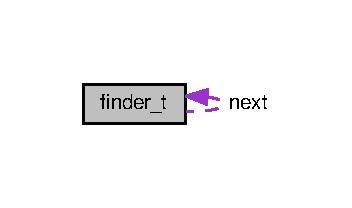
\includegraphics[width=188pt]{structfinder__t__coll__graph}
\end{center}
\end{figure}
\subsection*{Data Fields}
\begin{DoxyCompactItemize}
\item 
char $\ast$ \hyperlink{structfinder__t_aeac90097f29f7529968697163cea5c18}{filename}\hypertarget{structfinder__t_aeac90097f29f7529968697163cea5c18}{}\label{structfinder__t_aeac90097f29f7529968697163cea5c18}

\begin{DoxyCompactList}\small\item\em Found file name. \end{DoxyCompactList}\item 
struct \hyperlink{structfinder__t}{finder\+\_\+t} $\ast$ \hyperlink{structfinder__t_a7db9cac9324009990f14b7f84bf47d3c}{next}\hypertarget{structfinder__t_a7db9cac9324009990f14b7f84bf47d3c}{}\label{structfinder__t_a7db9cac9324009990f14b7f84bf47d3c}

\begin{DoxyCompactList}\small\item\em Next in the chain. \end{DoxyCompactList}\end{DoxyCompactItemize}


\subsection{Detailed Description}
A chained list of found file names. 

Definition at line 19 of file finder.\+h.



The documentation for this struct was generated from the following file\+:\begin{DoxyCompactItemize}
\item 
\hyperlink{finder_8h}{finder.\+h}\end{DoxyCompactItemize}

\hypertarget{structio__file__list}{}\section{io\+\_\+file\+\_\+list Struct Reference}
\label{structio__file__list}\index{io\+\_\+file\+\_\+list@{io\+\_\+file\+\_\+list}}
\subsection*{Data Fields}
\begin{DoxyCompactItemize}
\item 
char {\bfseries files} \mbox{[}I\+O\+\_\+\+D\+I\+R\+\_\+\+M\+A\+X\+\_\+\+F\+I\+L\+ES\mbox{]}\mbox{[}I\+O\+\_\+\+P\+A\+T\+H\+\_\+\+M\+A\+X\+\_\+\+S\+I\+ZE\mbox{]}\hypertarget{structio__file__list_aea2e7d487e7a0ce1737212bb7679dbcc}{}\label{structio__file__list_aea2e7d487e7a0ce1737212bb7679dbcc}

\item 
size\+\_\+t {\bfseries count}\hypertarget{structio__file__list_a76d971a3c552bc58ba9f0d5fceae9806}{}\label{structio__file__list_a76d971a3c552bc58ba9f0d5fceae9806}

\end{DoxyCompactItemize}


\subsection{Detailed Description}


Definition at line 17 of file io.\+h.



The documentation for this struct was generated from the following file\+:\begin{DoxyCompactItemize}
\item 
/home/claudio/git/smart-\/folder/src/io.\+h\end{DoxyCompactItemize}

\hypertarget{structparser__t}{}\section{parser\+\_\+t Struct Reference}
\label{structparser__t}\index{parser\+\_\+t@{parser\+\_\+t}}


Formal expression representation.  




{\ttfamily \#include $<$parser.\+h$>$}



Collaboration diagram for parser\+\_\+t\+:\nopagebreak
\begin{figure}[H]
\begin{center}
\leavevmode
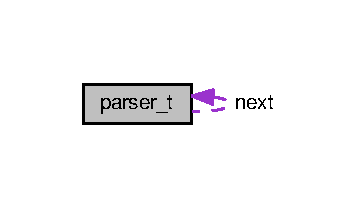
\includegraphics[width=172pt]{structparser__t__coll__graph}
\end{center}
\end{figure}
\subsection*{Data Fields}
\begin{DoxyCompactItemize}
\item 
\hyperlink{parser_8h_a4dcbe7148b91f50b0e7f3e08e780861d}{parser\+\_\+crit\+\_\+t} \hyperlink{structparser__t_af8e04406eee9097a92118be27b07eff7}{crit}
\begin{DoxyCompactList}\small\item\em The criteria for the token. \end{DoxyCompactList}\item 
void $\ast$ \hyperlink{structparser__t_a0f61d63b009d0880a89c843bd50d8d76}{value}
\begin{DoxyCompactList}\small\item\em The value of the criteria, the type depend on the type of \textquotesingle{}crit\textquotesingle{}. \end{DoxyCompactList}\item 
\hyperlink{parser_8h_ac721d0db2049edef01e62a2e63ff0472}{parser\+\_\+comp\+\_\+t} \hyperlink{structparser__t_a7bc05cec4ebb98215d11f1f354450f3d}{comp}
\begin{DoxyCompactList}\small\item\em The comparison to be used when evaluating the expression validity. \end{DoxyCompactList}\item 
struct \hyperlink{structparser__t}{parser\+\_\+t} $\ast$ \hyperlink{structparser__t_a044a5d882012dfdd9ea5e4f3a98fd8a2}{next}\hypertarget{structparser__t_a044a5d882012dfdd9ea5e4f3a98fd8a2}{}\label{structparser__t_a044a5d882012dfdd9ea5e4f3a98fd8a2}

\begin{DoxyCompactList}\small\item\em The next token in the expression. \end{DoxyCompactList}\end{DoxyCompactItemize}


\subsection{Detailed Description}
Formal expression representation. 

Contains the formal representation of the parsed expression in a ordered chained list. Each instance contains the information about a parsed expression token and the pointer to the {\ttfamily next} parsed expression token.

The order of the tokens in the chained list is not the same as the in the original string representation. Is has been reordered to encoded the priority of the operators and parenthesis in a infix notation 

Definition at line 71 of file parser.\+h.



\subsection{Field Documentation}
\index{parser\+\_\+t@{parser\+\_\+t}!comp@{comp}}
\index{comp@{comp}!parser\+\_\+t@{parser\+\_\+t}}
\subsubsection[{\texorpdfstring{comp}{comp}}]{\setlength{\rightskip}{0pt plus 5cm}{\bf parser\+\_\+comp\+\_\+t} comp}\hypertarget{structparser__t_a7bc05cec4ebb98215d11f1f354450f3d}{}\label{structparser__t_a7bc05cec4ebb98215d11f1f354450f3d}


The comparison to be used when evaluating the expression validity. 


\begin{DoxyItemize}
\item e.\+g. the {\ttfamily +} in the exp {\ttfamily -\/\+S\+I\+ZE +20}
\end{DoxyItemize}

\begin{DoxySeeAlso}{See also}
\hyperlink{parser_8h_ac721d0db2049edef01e62a2e63ff0472}{parser\+\_\+comp\+\_\+t} 
\end{DoxySeeAlso}


Definition at line 89 of file parser.\+h.

\index{parser\+\_\+t@{parser\+\_\+t}!crit@{crit}}
\index{crit@{crit}!parser\+\_\+t@{parser\+\_\+t}}
\subsubsection[{\texorpdfstring{crit}{crit}}]{\setlength{\rightskip}{0pt plus 5cm}{\bf parser\+\_\+crit\+\_\+t} crit}\hypertarget{structparser__t_af8e04406eee9097a92118be27b07eff7}{}\label{structparser__t_af8e04406eee9097a92118be27b07eff7}


The criteria for the token. 


\begin{DoxyItemize}
\item e.\+g. the {\ttfamily S\+I\+ZE} in the exp {\ttfamily -\/\+S\+I\+ZE +20}
\end{DoxyItemize}

\begin{DoxySeeAlso}{See also}
\hyperlink{parser_8h_a4dcbe7148b91f50b0e7f3e08e780861d}{parser\+\_\+crit\+\_\+t} 
\end{DoxySeeAlso}


Definition at line 77 of file parser.\+h.

\index{parser\+\_\+t@{parser\+\_\+t}!value@{value}}
\index{value@{value}!parser\+\_\+t@{parser\+\_\+t}}
\subsubsection[{\texorpdfstring{value}{value}}]{\setlength{\rightskip}{0pt plus 5cm}void$\ast$ value}\hypertarget{structparser__t_a0f61d63b009d0880a89c843bd50d8d76}{}\label{structparser__t_a0f61d63b009d0880a89c843bd50d8d76}


The value of the criteria, the type depend on the type of \textquotesingle{}crit\textquotesingle{}. 


\begin{DoxyItemize}
\item e.\+g. the {\ttfamily 20} in the exp {\ttfamily -\/\+S\+I\+ZE +20}
\end{DoxyItemize}

\begin{DoxySeeAlso}{See also}
\hyperlink{parser_8h_a4dcbe7148b91f50b0e7f3e08e780861d}{parser\+\_\+crit\+\_\+t} 
\end{DoxySeeAlso}


Definition at line 83 of file parser.\+h.



The documentation for this struct was generated from the following file\+:\begin{DoxyCompactItemize}
\item 
\hyperlink{parser_8h}{parser.\+h}\end{DoxyCompactItemize}

\hypertarget{structsearchfolder__t}{}\section{searchfolder\+\_\+t Struct Reference}
\label{structsearchfolder__t}\index{searchfolder\+\_\+t@{searchfolder\+\_\+t}}


Collaboration diagram for searchfolder\+\_\+t\+:\nopagebreak
\begin{figure}[H]
\begin{center}
\leavevmode
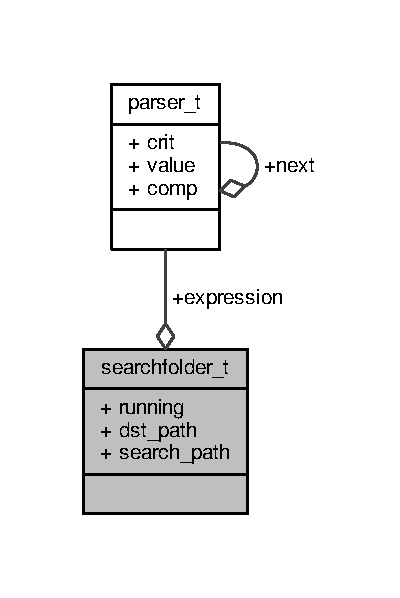
\includegraphics[width=185pt]{structsearchfolder__t__coll__graph}
\end{center}
\end{figure}
\subsection*{Data Fields}
\begin{DoxyCompactItemize}
\item 
bool {\bfseries running}\hypertarget{structsearchfolder__t_a36f7b6be7108281af77939ceaec42fd6}{}\label{structsearchfolder__t_a36f7b6be7108281af77939ceaec42fd6}

\item 
char $\ast$ {\bfseries dst\+\_\+path}\hypertarget{structsearchfolder__t_a74a7cec2bc63610109c58ef392d14e27}{}\label{structsearchfolder__t_a74a7cec2bc63610109c58ef392d14e27}

\item 
char $\ast$ {\bfseries search\+\_\+path}\hypertarget{structsearchfolder__t_a614ce96a64fa528698e05ce10070efe9}{}\label{structsearchfolder__t_a614ce96a64fa528698e05ce10070efe9}

\item 
\hyperlink{structparser__t}{parser\+\_\+t} $\ast$ {\bfseries expression}\hypertarget{structsearchfolder__t_a37eed245f4d8beb45412f8ba904643b2}{}\label{structsearchfolder__t_a37eed245f4d8beb45412f8ba904643b2}

\end{DoxyCompactItemize}


\subsection{Detailed Description}


Definition at line 11 of file searchfolder.\+c.



The documentation for this struct was generated from the following file\+:\begin{DoxyCompactItemize}
\item 
/home/claudio/git/smart-\/folder/src/searchfolder.\+c\end{DoxyCompactItemize}

\chapter{File Documentation}
\hypertarget{parser_8c}{}\section{parser.\+c File Reference}
\label{parser_8c}\index{parser.\+c@{parser.\+c}}


Parses a string expression and return a formal representation.  


{\ttfamily \#include $<$string.\+h$>$}\\*
{\ttfamily \#include $<$stdlib.\+h$>$}\\*
{\ttfamily \#include $<$math.\+h$>$}\\*
{\ttfamily \#include $<$pwd.\+h$>$}\\*
{\ttfamily \#include $<$grp.\+h$>$}\\*
{\ttfamily \#include \char`\"{}parser.\+h\char`\"{}}\\*
{\ttfamily \#include \char`\"{}logger.\+h\char`\"{}}\\*
Include dependency graph for parser.\+c\+:\nopagebreak
\begin{figure}[H]
\begin{center}
\leavevmode
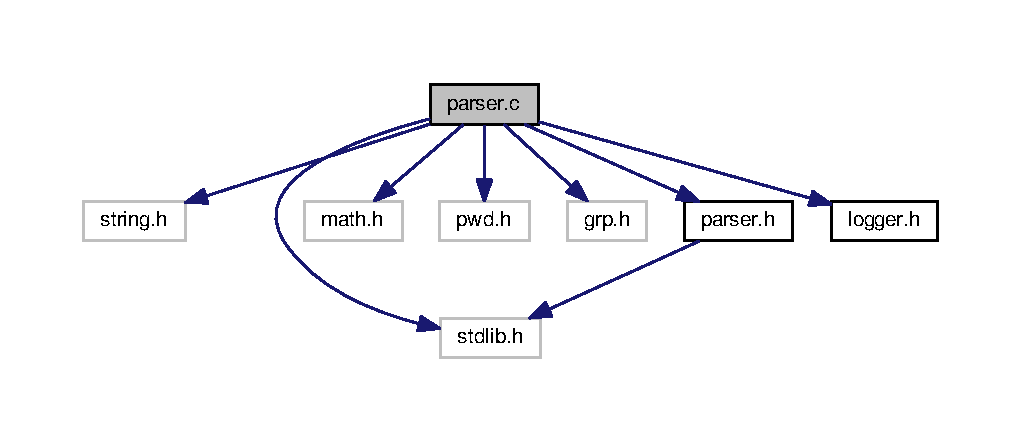
\includegraphics[width=350pt]{parser_8c__incl}
\end{center}
\end{figure}
\subsection*{Macros}
\begin{DoxyCompactItemize}
\item 
\#define \hyperlink{parser_8c_a20f8a4e237e6918372da5e1aec3426c8}{C\+R\+I\+T\+E\+R\+I\+A\+\_\+\+C\+O\+U\+NT}~8
\begin{DoxyCompactList}\small\item\em Number of criteria belonging to the C\+R\+I\+T\+E\+R\+IA criteria type. \end{DoxyCompactList}\item 
\#define \hyperlink{parser_8c_aa072d0e80f3a95589705ecb2000fbe03}{O\+P\+E\+R\+A\+T\+O\+R\+S\+\_\+\+C\+O\+U\+NT}~5
\begin{DoxyCompactList}\small\item\em Number of criteria belonging to the O\+P\+E\+R\+A\+T\+OR criteria type. \end{DoxyCompactList}\item 
\#define \hyperlink{parser_8c_af5463cdb2a7f99c341f1c577749bd411}{M\+I\+N\+\_\+\+OP}~\textquotesingle{}-\/\textquotesingle{}
\begin{DoxyCompactList}\small\item\em Symbol for M\+IN comparison operator. \end{DoxyCompactList}\item 
\#define \hyperlink{parser_8c_af82bd7ec45d35820df88615c2eeb716e}{M\+A\+X\+\_\+\+OP}~\textquotesingle{}+\textquotesingle{}
\begin{DoxyCompactList}\small\item\em Symbol for M\+AX comparison operator. \end{DoxyCompactList}\end{DoxyCompactItemize}
\subsection*{Typedefs}
\begin{DoxyCompactItemize}
\item 
typedef \hyperlink{structparser__t}{parser\+\_\+t} $\ast$($\ast$ \hyperlink{parser_8c_ac724e9bd64934497a297ce90c3d1033e}{parse\+\_\+fn\+\_\+t}) (char $\ast$)\hypertarget{parser_8c_ac724e9bd64934497a297ce90c3d1033e}{}\label{parser_8c_ac724e9bd64934497a297ce90c3d1033e}

\begin{DoxyCompactList}\small\item\em Function pointer for token parser functions. \end{DoxyCompactList}\end{DoxyCompactItemize}
\subsection*{Functions}
\begin{DoxyCompactItemize}
\item 
static \hyperlink{structparser__t}{parser\+\_\+t} $\ast$ \hyperlink{parser_8c_a47b4c85a9d0396d24026547068b0f819}{parse\+\_\+value} (char $\ast$argv, \hyperlink{parser_8h_a4dcbe7148b91f50b0e7f3e08e780861d}{parser\+\_\+crit\+\_\+t} \hyperlink{parser_8c_a763a1adefb032e8ebd05b1acfe86d7f8}{criteria})
\begin{DoxyCompactList}\small\item\em Parses an expression value and evaluates value prefix. \end{DoxyCompactList}\item 
static \hyperlink{structparser__t}{parser\+\_\+t} $\ast$ \hyperlink{parser_8c_afe16485de5b439108774ac9009d8516c}{parse\+\_\+name} (char $\ast$argv)
\begin{DoxyCompactList}\small\item\em Parses N\+A\+ME criteria. \end{DoxyCompactList}\item 
static \hyperlink{structparser__t}{parser\+\_\+t} $\ast$ \hyperlink{parser_8c_aa9408aed6d30c7d254d95aae15594ff8}{parse\+\_\+group} (char $\ast$argv)
\begin{DoxyCompactList}\small\item\em Parses G\+R\+O\+UP criteria. \end{DoxyCompactList}\item 
static \hyperlink{structparser__t}{parser\+\_\+t} $\ast$ \hyperlink{parser_8c_a40f898b4a8a3f8a4f892f309d3568fa0}{parse\+\_\+user} (char $\ast$argv)
\begin{DoxyCompactList}\small\item\em Parses U\+S\+ER criteria. \end{DoxyCompactList}\item 
static \hyperlink{structparser__t}{parser\+\_\+t} $\ast$ \hyperlink{parser_8c_a62a2c8d6d820d3c8ddada3f9e3db3c81}{parse\+\_\+perm} (char $\ast$argv)
\begin{DoxyCompactList}\small\item\em Parses P\+E\+RM criteria. \end{DoxyCompactList}\item 
static char \hyperlink{parser_8c_a1855729ff4d2fb0fca6e84e89469eff9}{parse\+\_\+exp\+\_\+unity} (char $\ast$exp)
\begin{DoxyCompactList}\small\item\em Extracts the unity character of the value. \end{DoxyCompactList}\item 
static \hyperlink{structparser__t}{parser\+\_\+t} $\ast$ \hyperlink{parser_8c_aee42f858f9459f7affc7b3c95afd7b4d}{parse\+\_\+size} (char $\ast$argv)
\begin{DoxyCompactList}\small\item\em Parses S\+I\+ZE criteria. \end{DoxyCompactList}\item 
static \hyperlink{structparser__t}{parser\+\_\+t} $\ast$ \hyperlink{parser_8c_ab6c6e61351a1fd8002d093f890617d17}{parse\+\_\+time} (char $\ast$argv, \hyperlink{parser_8h_a4dcbe7148b91f50b0e7f3e08e780861d}{parser\+\_\+crit\+\_\+t} \hyperlink{parser_8c_a763a1adefb032e8ebd05b1acfe86d7f8}{criteria})
\begin{DoxyCompactList}\small\item\em Parses T\+I\+ME criteria. \end{DoxyCompactList}\item 
static \hyperlink{structparser__t}{parser\+\_\+t} $\ast$ \hyperlink{parser_8c_a93ea7c5840f4c1f42a6084459ed86cd3}{parse\+\_\+atime} (char $\ast$argv)
\begin{DoxyCompactList}\small\item\em Parses A\+T\+I\+ME criteria. \end{DoxyCompactList}\item 
static \hyperlink{structparser__t}{parser\+\_\+t} $\ast$ \hyperlink{parser_8c_a382db2f7e93c5300665f4460c58f34c8}{parse\+\_\+ctime} (char $\ast$argv)
\begin{DoxyCompactList}\small\item\em Parses C\+T\+I\+ME criteria. \end{DoxyCompactList}\item 
static \hyperlink{structparser__t}{parser\+\_\+t} $\ast$ \hyperlink{parser_8c_a1f92a14247cf2cfefef84007d82e3463}{parse\+\_\+mtime} (char $\ast$argv)
\begin{DoxyCompactList}\small\item\em Parses M\+T\+I\+ME criteria. \end{DoxyCompactList}\item 
static \hyperlink{structparser__t}{parser\+\_\+t} $\ast$ \hyperlink{parser_8c_a07a71747919666059eb75bde7432986a}{parse\+\_\+op} (\hyperlink{parser_8h_a4dcbe7148b91f50b0e7f3e08e780861d}{parser\+\_\+crit\+\_\+t} op)
\begin{DoxyCompactList}\small\item\em Parses operator. \end{DoxyCompactList}\item 
static char $\ast$ \hyperlink{parser_8c_acc7b54ce1cab8f6c383107595d1283c3}{operator\mbox{[}\+O\+P\+E\+R\+A\+T\+O\+R\+S\+\_\+\+C\+O\+U\+N\+T\mbox{]}=\{\char`\"{}-\/not\char`\"{},\char`\"{}-\/and\char`\"{},\char`\"{}-\/or\char`\"{},\char`\"{}} (\char`\"{}, \char`\"{})\char`\"{}\}
\begin{DoxyCompactList}\small\item\em List of operators and parenthesis string tokens. \end{DoxyCompactList}\item 
static \hyperlink{structparser__t}{parser\+\_\+t} $\ast$ \hyperlink{parser_8c_a57b8f2ef8e0428becf3401c85126b0cb}{parse\+\_\+token} (char $\ast$$\ast$expression\mbox{[}$\,$\mbox{]}, size\+\_\+t $\ast$size)
\begin{DoxyCompactList}\small\item\em Parses a token in the expression. \end{DoxyCompactList}\item 
static void \hyperlink{parser_8c_a1daa9e72258e5f6424fffab656b42b36}{move\+\_\+token} (\hyperlink{structparser__t}{parser\+\_\+t} $\ast$$\ast$to, \hyperlink{structparser__t}{parser\+\_\+t} $\ast$$\ast$from)\hypertarget{parser_8c_a1daa9e72258e5f6424fffab656b42b36}{}\label{parser_8c_a1daa9e72258e5f6424fffab656b42b36}

\begin{DoxyCompactList}\small\item\em Helper method to move the top {\ttfamily \hyperlink{structparser__t}{parser\+\_\+t}} from a stack to another. \end{DoxyCompactList}\item 
static \hyperlink{structparser__t}{parser\+\_\+t} $\ast$ \hyperlink{parser_8c_adf95518fbae3d3bc7a44815945197e33}{parser\+\_\+infix\+\_\+notation} (\hyperlink{structparser__t}{parser\+\_\+t} $\ast$exp)
\begin{DoxyCompactList}\small\item\em Orders a chained list of {\ttfamily \hyperlink{structparser__t}{parser\+\_\+t}}. \end{DoxyCompactList}\item 
\hyperlink{structparser__t}{parser\+\_\+t} $\ast$ \hyperlink{parser_8c_a570f8d50af35e4863518a619ef74d501}{parser\+\_\+parse} (char $\ast$expression\mbox{[}$\,$\mbox{]}, size\+\_\+t size)
\begin{DoxyCompactList}\small\item\em Parses the string expression, converting it to a {\ttfamily \hyperlink{structparser__t}{parser\+\_\+t}} representation. \end{DoxyCompactList}\item 
void \hyperlink{parser_8c_a680ceeada57c4645e365ba1745d41181}{parser\+\_\+free} (\hyperlink{structparser__t}{parser\+\_\+t} $\ast$expression)
\begin{DoxyCompactList}\small\item\em Frees the memory allocated for a {\ttfamily \hyperlink{structparser__t}{parser\+\_\+t}} instance. \end{DoxyCompactList}\end{DoxyCompactItemize}
\subsection*{Variables}
\begin{DoxyCompactItemize}
\item 
static \hyperlink{structparser__t}{parser\+\_\+t} char $\ast$ \hyperlink{parser_8c_a763a1adefb032e8ebd05b1acfe86d7f8}{criteria} \mbox{[}\hyperlink{validator_8c_a20f8a4e237e6918372da5e1aec3426c8}{C\+R\+I\+T\+E\+R\+I\+A\+\_\+\+C\+O\+U\+NT}\mbox{]} = \{\char`\"{}-\/name\char`\"{}, \char`\"{}-\/group\char`\"{}, \char`\"{}-\/user\char`\"{}, \char`\"{}-\/perm\char`\"{}, \char`\"{}-\/size\char`\"{}, \char`\"{}-\/atime\char`\"{}, \char`\"{}-\/ctime\char`\"{}, \char`\"{}-\/mtime\char`\"{}\}
\begin{DoxyCompactList}\small\item\em List of criteria string tokens. \end{DoxyCompactList}\item 
static \hyperlink{parser_8c_ac724e9bd64934497a297ce90c3d1033e}{parse\+\_\+fn\+\_\+t} \hyperlink{parser_8c_ab8af9d65906b7a6d27351b73bf215518}{criteria\+\_\+type} \mbox{[}\hyperlink{validator_8c_a20f8a4e237e6918372da5e1aec3426c8}{C\+R\+I\+T\+E\+R\+I\+A\+\_\+\+C\+O\+U\+NT}\mbox{]}
\begin{DoxyCompactList}\small\item\em List of of criteria parsing functions. \end{DoxyCompactList}\item 
static \hyperlink{parser_8h_a4dcbe7148b91f50b0e7f3e08e780861d}{parser\+\_\+crit\+\_\+t} \hyperlink{parser_8c_a40fc071998f92796527a47358d5ec42b}{operator\+\_\+type} \mbox{[}\hyperlink{parser_8c_aa072d0e80f3a95589705ecb2000fbe03}{O\+P\+E\+R\+A\+T\+O\+R\+S\+\_\+\+C\+O\+U\+NT}\mbox{]} = \{N\+OT, A\+ND, OR, L\+P\+A\+R\+E\+N\+T\+H\+E\+S\+IS, R\+P\+A\+R\+E\+N\+T\+H\+E\+S\+IS\}
\begin{DoxyCompactList}\small\item\em List of operators and parenthesis matching the operators in {\ttfamily operator}. \end{DoxyCompactList}\end{DoxyCompactItemize}


\subsection{Detailed Description}
Parses a string expression and return a formal representation. 

Full unit test coverage 

\subsection{Macro Definition Documentation}
\index{parser.\+c@{parser.\+c}!C\+R\+I\+T\+E\+R\+I\+A\+\_\+\+C\+O\+U\+NT@{C\+R\+I\+T\+E\+R\+I\+A\+\_\+\+C\+O\+U\+NT}}
\index{C\+R\+I\+T\+E\+R\+I\+A\+\_\+\+C\+O\+U\+NT@{C\+R\+I\+T\+E\+R\+I\+A\+\_\+\+C\+O\+U\+NT}!parser.\+c@{parser.\+c}}
\subsubsection[{\texorpdfstring{C\+R\+I\+T\+E\+R\+I\+A\+\_\+\+C\+O\+U\+NT}{CRITERIA_COUNT}}]{\setlength{\rightskip}{0pt plus 5cm}\#define C\+R\+I\+T\+E\+R\+I\+A\+\_\+\+C\+O\+U\+NT~8}\hypertarget{parser_8c_a20f8a4e237e6918372da5e1aec3426c8}{}\label{parser_8c_a20f8a4e237e6918372da5e1aec3426c8}


Number of criteria belonging to the C\+R\+I\+T\+E\+R\+IA criteria type. 

\begin{DoxySeeAlso}{See also}
\hyperlink{parser_8h_a4dcbe7148b91f50b0e7f3e08e780861d}{parser\+\_\+crit\+\_\+t} 

\hyperlink{parser_8h_a32088e9f194a33e050822b8c536e03cb}{parser\+\_\+crit\+\_\+type\+\_\+t} 
\end{DoxySeeAlso}


Definition at line 19 of file parser.\+c.

\index{parser.\+c@{parser.\+c}!M\+A\+X\+\_\+\+OP@{M\+A\+X\+\_\+\+OP}}
\index{M\+A\+X\+\_\+\+OP@{M\+A\+X\+\_\+\+OP}!parser.\+c@{parser.\+c}}
\subsubsection[{\texorpdfstring{M\+A\+X\+\_\+\+OP}{MAX_OP}}]{\setlength{\rightskip}{0pt plus 5cm}\#define M\+A\+X\+\_\+\+OP~\textquotesingle{}+\textquotesingle{}}\hypertarget{parser_8c_af82bd7ec45d35820df88615c2eeb716e}{}\label{parser_8c_af82bd7ec45d35820df88615c2eeb716e}


Symbol for M\+AX comparison operator. 

\begin{DoxySeeAlso}{See also}
\hyperlink{parser_8h_ac721d0db2049edef01e62a2e63ff0472}{parser\+\_\+comp\+\_\+t} 
\end{DoxySeeAlso}


Definition at line 30 of file parser.\+c.

\index{parser.\+c@{parser.\+c}!M\+I\+N\+\_\+\+OP@{M\+I\+N\+\_\+\+OP}}
\index{M\+I\+N\+\_\+\+OP@{M\+I\+N\+\_\+\+OP}!parser.\+c@{parser.\+c}}
\subsubsection[{\texorpdfstring{M\+I\+N\+\_\+\+OP}{MIN_OP}}]{\setlength{\rightskip}{0pt plus 5cm}\#define M\+I\+N\+\_\+\+OP~\textquotesingle{}-\/\textquotesingle{}}\hypertarget{parser_8c_af5463cdb2a7f99c341f1c577749bd411}{}\label{parser_8c_af5463cdb2a7f99c341f1c577749bd411}


Symbol for M\+IN comparison operator. 

\begin{DoxySeeAlso}{See also}
\hyperlink{parser_8h_ac721d0db2049edef01e62a2e63ff0472}{parser\+\_\+comp\+\_\+t} 
\end{DoxySeeAlso}


Definition at line 28 of file parser.\+c.

\index{parser.\+c@{parser.\+c}!O\+P\+E\+R\+A\+T\+O\+R\+S\+\_\+\+C\+O\+U\+NT@{O\+P\+E\+R\+A\+T\+O\+R\+S\+\_\+\+C\+O\+U\+NT}}
\index{O\+P\+E\+R\+A\+T\+O\+R\+S\+\_\+\+C\+O\+U\+NT@{O\+P\+E\+R\+A\+T\+O\+R\+S\+\_\+\+C\+O\+U\+NT}!parser.\+c@{parser.\+c}}
\subsubsection[{\texorpdfstring{O\+P\+E\+R\+A\+T\+O\+R\+S\+\_\+\+C\+O\+U\+NT}{OPERATORS_COUNT}}]{\setlength{\rightskip}{0pt plus 5cm}\#define O\+P\+E\+R\+A\+T\+O\+R\+S\+\_\+\+C\+O\+U\+NT~5}\hypertarget{parser_8c_aa072d0e80f3a95589705ecb2000fbe03}{}\label{parser_8c_aa072d0e80f3a95589705ecb2000fbe03}


Number of criteria belonging to the O\+P\+E\+R\+A\+T\+OR criteria type. 

\begin{DoxySeeAlso}{See also}
\hyperlink{parser_8h_a4dcbe7148b91f50b0e7f3e08e780861d}{parser\+\_\+crit\+\_\+t} 

\hyperlink{parser_8h_a32088e9f194a33e050822b8c536e03cb}{parser\+\_\+crit\+\_\+type\+\_\+t} 
\end{DoxySeeAlso}


Definition at line 25 of file parser.\+c.



\subsection{Function Documentation}
\index{parser.\+c@{parser.\+c}!operator\mbox{[}\+O\+P\+E\+R\+A\+T\+O\+R\+S\+\_\+\+C\+O\+U\+N\+T\mbox{]}=\lcurly{}\char`\"{}-\/not\char`\"{},\char`\"{}-\/and\char`\"{},\char`\"{}-\/or\char`\"{},\char`\"{}@{operator[O\+P\+E\+R\+A\+T\+O\+R\+S\+\_\+\+C\+O\+U\+NT]=\lcurly{}""-\/not"",""-\/and"",""-\/or"",""}}
\index{operator\mbox{[}\+O\+P\+E\+R\+A\+T\+O\+R\+S\+\_\+\+C\+O\+U\+N\+T\mbox{]}=\lcurly{}\char`\"{}-\/not\char`\"{},\char`\"{}-\/and\char`\"{},\char`\"{}-\/or\char`\"{},\char`\"{}@{operator[O\+P\+E\+R\+A\+T\+O\+R\+S\+\_\+\+C\+O\+U\+NT]=\lcurly{}""-\/not"",""-\/and"",""-\/or"",""}!parser.\+c@{parser.\+c}}
\subsubsection[{\texorpdfstring{operator[O\+P\+E\+R\+A\+T\+O\+R\+S\+\_\+\+C\+O\+U\+NT]=\lcurly{}""-\/not"",""-\/and"",""-\/or"",""("", "")""\rcurly{}}{operator[OPERATORS_COUNT]=\{"-not","-and","-or","(", ")"\}}}]{\setlength{\rightskip}{0pt plus 5cm}static char$\ast$ operator\mbox{[}{\bf O\+P\+E\+R\+A\+T\+O\+R\+S\+\_\+\+C\+O\+U\+NT}\mbox{]}=\{\char`\"{}-\/not\char`\"{},\char`\"{}-\/and\char`\"{},\char`\"{}-\/or\char`\"{},\char`\"{} (
\begin{DoxyParamCaption}
\item[{\char`\"{}}]{, }
\item[{\char`\"{}}]{}
\end{DoxyParamCaption}
)\hspace{0.3cm}{\ttfamily [static]}}\hypertarget{parser_8c_acc7b54ce1cab8f6c383107595d1283c3}{}\label{parser_8c_acc7b54ce1cab8f6c383107595d1283c3}


List of operators and parenthesis string tokens. 

Used for recognizing then in the given expression.

\begin{DoxySeeAlso}{See also}
\hyperlink{parser_8h_a4dcbe7148b91f50b0e7f3e08e780861d}{parser\+\_\+crit\+\_\+t} 

\hyperlink{parser_8c_a57b8f2ef8e0428becf3401c85126b0cb}{parse\+\_\+token} 
\end{DoxySeeAlso}
\index{parser.\+c@{parser.\+c}!parse\+\_\+atime@{parse\+\_\+atime}}
\index{parse\+\_\+atime@{parse\+\_\+atime}!parser.\+c@{parser.\+c}}
\subsubsection[{\texorpdfstring{parse\+\_\+atime(char $\ast$argv)}{parse_atime(char *argv)}}]{\setlength{\rightskip}{0pt plus 5cm}static {\bf parser\+\_\+t}$\ast$ parse\+\_\+atime (
\begin{DoxyParamCaption}
\item[{char $\ast$}]{argv}
\end{DoxyParamCaption}
)\hspace{0.3cm}{\ttfamily [static]}}\hypertarget{parser_8c_a93ea7c5840f4c1f42a6084459ed86cd3}{}\label{parser_8c_a93ea7c5840f4c1f42a6084459ed86cd3}


Parses A\+T\+I\+ME criteria. 



Definition at line 199 of file parser.\+c.

\index{parser.\+c@{parser.\+c}!parse\+\_\+ctime@{parse\+\_\+ctime}}
\index{parse\+\_\+ctime@{parse\+\_\+ctime}!parser.\+c@{parser.\+c}}
\subsubsection[{\texorpdfstring{parse\+\_\+ctime(char $\ast$argv)}{parse_ctime(char *argv)}}]{\setlength{\rightskip}{0pt plus 5cm}static {\bf parser\+\_\+t}$\ast$ parse\+\_\+ctime (
\begin{DoxyParamCaption}
\item[{char $\ast$}]{argv}
\end{DoxyParamCaption}
)\hspace{0.3cm}{\ttfamily [static]}}\hypertarget{parser_8c_a382db2f7e93c5300665f4460c58f34c8}{}\label{parser_8c_a382db2f7e93c5300665f4460c58f34c8}


Parses C\+T\+I\+ME criteria. 



Definition at line 204 of file parser.\+c.

\index{parser.\+c@{parser.\+c}!parse\+\_\+exp\+\_\+unity@{parse\+\_\+exp\+\_\+unity}}
\index{parse\+\_\+exp\+\_\+unity@{parse\+\_\+exp\+\_\+unity}!parser.\+c@{parser.\+c}}
\subsubsection[{\texorpdfstring{parse\+\_\+exp\+\_\+unity(char $\ast$exp)}{parse_exp_unity(char *exp)}}]{\setlength{\rightskip}{0pt plus 5cm}static char parse\+\_\+exp\+\_\+unity (
\begin{DoxyParamCaption}
\item[{char $\ast$}]{exp}
\end{DoxyParamCaption}
)\hspace{0.3cm}{\ttfamily [static]}}\hypertarget{parser_8c_a1855729ff4d2fb0fca6e84e89469eff9}{}\label{parser_8c_a1855729ff4d2fb0fca6e84e89469eff9}


Extracts the unity character of the value. 


\begin{DoxyParams}{Parameters}
{\em exp} & The criteria value \\
\hline
\end{DoxyParams}
\begin{DoxyReturn}{Returns}
The unity character if found. 0 If no unity character found. -\/1 if error 
\end{DoxyReturn}


Definition at line 116 of file parser.\+c.

\index{parser.\+c@{parser.\+c}!parse\+\_\+group@{parse\+\_\+group}}
\index{parse\+\_\+group@{parse\+\_\+group}!parser.\+c@{parser.\+c}}
\subsubsection[{\texorpdfstring{parse\+\_\+group(char $\ast$argv)}{parse_group(char *argv)}}]{\setlength{\rightskip}{0pt plus 5cm}static {\bf parser\+\_\+t}$\ast$ parse\+\_\+group (
\begin{DoxyParamCaption}
\item[{char $\ast$}]{argv}
\end{DoxyParamCaption}
)\hspace{0.3cm}{\ttfamily [static]}}\hypertarget{parser_8c_aa9408aed6d30c7d254d95aae15594ff8}{}\label{parser_8c_aa9408aed6d30c7d254d95aae15594ff8}


Parses G\+R\+O\+UP criteria. 



Definition at line 62 of file parser.\+c.

\index{parser.\+c@{parser.\+c}!parse\+\_\+mtime@{parse\+\_\+mtime}}
\index{parse\+\_\+mtime@{parse\+\_\+mtime}!parser.\+c@{parser.\+c}}
\subsubsection[{\texorpdfstring{parse\+\_\+mtime(char $\ast$argv)}{parse_mtime(char *argv)}}]{\setlength{\rightskip}{0pt plus 5cm}static {\bf parser\+\_\+t}$\ast$ parse\+\_\+mtime (
\begin{DoxyParamCaption}
\item[{char $\ast$}]{argv}
\end{DoxyParamCaption}
)\hspace{0.3cm}{\ttfamily [static]}}\hypertarget{parser_8c_a1f92a14247cf2cfefef84007d82e3463}{}\label{parser_8c_a1f92a14247cf2cfefef84007d82e3463}


Parses M\+T\+I\+ME criteria. 



Definition at line 209 of file parser.\+c.

\index{parser.\+c@{parser.\+c}!parse\+\_\+name@{parse\+\_\+name}}
\index{parse\+\_\+name@{parse\+\_\+name}!parser.\+c@{parser.\+c}}
\subsubsection[{\texorpdfstring{parse\+\_\+name(char $\ast$argv)}{parse_name(char *argv)}}]{\setlength{\rightskip}{0pt plus 5cm}static {\bf parser\+\_\+t}$\ast$ parse\+\_\+name (
\begin{DoxyParamCaption}
\item[{char $\ast$}]{argv}
\end{DoxyParamCaption}
)\hspace{0.3cm}{\ttfamily [static]}}\hypertarget{parser_8c_afe16485de5b439108774ac9009d8516c}{}\label{parser_8c_afe16485de5b439108774ac9009d8516c}


Parses N\+A\+ME criteria. 



Definition at line 53 of file parser.\+c.

\index{parser.\+c@{parser.\+c}!parse\+\_\+op@{parse\+\_\+op}}
\index{parse\+\_\+op@{parse\+\_\+op}!parser.\+c@{parser.\+c}}
\subsubsection[{\texorpdfstring{parse\+\_\+op(parser\+\_\+crit\+\_\+t op)}{parse_op(parser_crit_t op)}}]{\setlength{\rightskip}{0pt plus 5cm}static {\bf parser\+\_\+t}$\ast$ parse\+\_\+op (
\begin{DoxyParamCaption}
\item[{{\bf parser\+\_\+crit\+\_\+t}}]{op}
\end{DoxyParamCaption}
)\hspace{0.3cm}{\ttfamily [static]}}\hypertarget{parser_8c_a07a71747919666059eb75bde7432986a}{}\label{parser_8c_a07a71747919666059eb75bde7432986a}


Parses operator. 



Definition at line 214 of file parser.\+c.

\index{parser.\+c@{parser.\+c}!parse\+\_\+perm@{parse\+\_\+perm}}
\index{parse\+\_\+perm@{parse\+\_\+perm}!parser.\+c@{parser.\+c}}
\subsubsection[{\texorpdfstring{parse\+\_\+perm(char $\ast$argv)}{parse_perm(char *argv)}}]{\setlength{\rightskip}{0pt plus 5cm}static {\bf parser\+\_\+t}$\ast$ parse\+\_\+perm (
\begin{DoxyParamCaption}
\item[{char $\ast$}]{argv}
\end{DoxyParamCaption}
)\hspace{0.3cm}{\ttfamily [static]}}\hypertarget{parser_8c_a62a2c8d6d820d3c8ddada3f9e3db3c81}{}\label{parser_8c_a62a2c8d6d820d3c8ddada3f9e3db3c81}


Parses P\+E\+RM criteria. 



Definition at line 98 of file parser.\+c.

\index{parser.\+c@{parser.\+c}!parse\+\_\+size@{parse\+\_\+size}}
\index{parse\+\_\+size@{parse\+\_\+size}!parser.\+c@{parser.\+c}}
\subsubsection[{\texorpdfstring{parse\+\_\+size(char $\ast$argv)}{parse_size(char *argv)}}]{\setlength{\rightskip}{0pt plus 5cm}static {\bf parser\+\_\+t}$\ast$ parse\+\_\+size (
\begin{DoxyParamCaption}
\item[{char $\ast$}]{argv}
\end{DoxyParamCaption}
)\hspace{0.3cm}{\ttfamily [static]}}\hypertarget{parser_8c_aee42f858f9459f7affc7b3c95afd7b4d}{}\label{parser_8c_aee42f858f9459f7affc7b3c95afd7b4d}


Parses S\+I\+ZE criteria. 



Definition at line 134 of file parser.\+c.

\index{parser.\+c@{parser.\+c}!parse\+\_\+time@{parse\+\_\+time}}
\index{parse\+\_\+time@{parse\+\_\+time}!parser.\+c@{parser.\+c}}
\subsubsection[{\texorpdfstring{parse\+\_\+time(char $\ast$argv, parser\+\_\+crit\+\_\+t criteria)}{parse_time(char *argv, parser_crit_t criteria)}}]{\setlength{\rightskip}{0pt plus 5cm}static {\bf parser\+\_\+t}$\ast$ parse\+\_\+time (
\begin{DoxyParamCaption}
\item[{char $\ast$}]{argv, }
\item[{{\bf parser\+\_\+crit\+\_\+t}}]{criteria}
\end{DoxyParamCaption}
)\hspace{0.3cm}{\ttfamily [static]}}\hypertarget{parser_8c_ab6c6e61351a1fd8002d093f890617d17}{}\label{parser_8c_ab6c6e61351a1fd8002d093f890617d17}


Parses T\+I\+ME criteria. 



Definition at line 167 of file parser.\+c.

\index{parser.\+c@{parser.\+c}!parse\+\_\+token@{parse\+\_\+token}}
\index{parse\+\_\+token@{parse\+\_\+token}!parser.\+c@{parser.\+c}}
\subsubsection[{\texorpdfstring{parse\+\_\+token(char $\ast$$\ast$expression[], size\+\_\+t $\ast$size)}{parse_token(char **expression[], size_t *size)}}]{\setlength{\rightskip}{0pt plus 5cm}static {\bf parser\+\_\+t}$\ast$ parse\+\_\+token (
\begin{DoxyParamCaption}
\item[{char $\ast$$\ast$}]{expression\mbox{[}$\,$\mbox{]}, }
\item[{size\+\_\+t $\ast$}]{size}
\end{DoxyParamCaption}
)\hspace{0.3cm}{\ttfamily [static]}}\hypertarget{parser_8c_a57b8f2ef8e0428becf3401c85126b0cb}{}\label{parser_8c_a57b8f2ef8e0428becf3401c85126b0cb}


Parses a token in the expression. 

The token in the expression in compared against {\ttfamily criteria} and {\ttfamily operator}. Once a token has been recognized, the corresponding function in {\ttfamily criteria\+\_\+type} or {\ttfamily parse\+\_\+op} is called.


\begin{DoxyParams}{Parameters}
{\em expression} & Pointer to the current token to be parsed \\
\hline
{\em size} & Current tokens left to be parsed \\
\hline
\end{DoxyParams}
\begin{DoxyReturn}{Returns}
The corresponding {\ttfamily \hyperlink{structparser__t}{parser\+\_\+t}} instance 
\end{DoxyReturn}


Definition at line 264 of file parser.\+c.

\index{parser.\+c@{parser.\+c}!parse\+\_\+user@{parse\+\_\+user}}
\index{parse\+\_\+user@{parse\+\_\+user}!parser.\+c@{parser.\+c}}
\subsubsection[{\texorpdfstring{parse\+\_\+user(char $\ast$argv)}{parse_user(char *argv)}}]{\setlength{\rightskip}{0pt plus 5cm}static {\bf parser\+\_\+t}$\ast$ parse\+\_\+user (
\begin{DoxyParamCaption}
\item[{char $\ast$}]{argv}
\end{DoxyParamCaption}
)\hspace{0.3cm}{\ttfamily [static]}}\hypertarget{parser_8c_a40f898b4a8a3f8a4f892f309d3568fa0}{}\label{parser_8c_a40f898b4a8a3f8a4f892f309d3568fa0}


Parses U\+S\+ER criteria. 



Definition at line 80 of file parser.\+c.

\index{parser.\+c@{parser.\+c}!parse\+\_\+value@{parse\+\_\+value}}
\index{parse\+\_\+value@{parse\+\_\+value}!parser.\+c@{parser.\+c}}
\subsubsection[{\texorpdfstring{parse\+\_\+value(char $\ast$argv, parser\+\_\+crit\+\_\+t criteria)}{parse_value(char *argv, parser_crit_t criteria)}}]{\setlength{\rightskip}{0pt plus 5cm}static {\bf parser\+\_\+t}$\ast$ parse\+\_\+value (
\begin{DoxyParamCaption}
\item[{char $\ast$}]{argv, }
\item[{{\bf parser\+\_\+crit\+\_\+t}}]{criteria}
\end{DoxyParamCaption}
)\hspace{0.3cm}{\ttfamily [static]}}\hypertarget{parser_8c_a47b4c85a9d0396d24026547068b0f819}{}\label{parser_8c_a47b4c85a9d0396d24026547068b0f819}


Parses an expression value and evaluates value prefix. 


\begin{DoxyParams}{Parameters}
{\em argv} & Argument for value token \\
\hline
{\em criteria} & The criteria type to use \\
\hline
\end{DoxyParams}
\begin{DoxyReturn}{Returns}
The resulting {\ttfamily \hyperlink{structparser__t}{parser\+\_\+t}}instance 
\end{DoxyReturn}


Definition at line 37 of file parser.\+c.

\index{parser.\+c@{parser.\+c}!parser\+\_\+free@{parser\+\_\+free}}
\index{parser\+\_\+free@{parser\+\_\+free}!parser.\+c@{parser.\+c}}
\subsubsection[{\texorpdfstring{parser\+\_\+free(parser\+\_\+t $\ast$expression)}{parser_free(parser_t *expression)}}]{\setlength{\rightskip}{0pt plus 5cm}void parser\+\_\+free (
\begin{DoxyParamCaption}
\item[{{\bf parser\+\_\+t} $\ast$}]{expression}
\end{DoxyParamCaption}
)}\hypertarget{parser_8c_a680ceeada57c4645e365ba1745d41181}{}\label{parser_8c_a680ceeada57c4645e365ba1745d41181}


Frees the memory allocated for a {\ttfamily \hyperlink{structparser__t}{parser\+\_\+t}} instance. 

\begin{DoxySeeAlso}{See also}
\hyperlink{structparser__t}{parser\+\_\+t} 
\end{DoxySeeAlso}

\begin{DoxyParams}{Parameters}
{\em expression} & The `parser\+\_\+t instance to free \\
\hline
\end{DoxyParams}


Definition at line 366 of file parser.\+c.

\index{parser.\+c@{parser.\+c}!parser\+\_\+infix\+\_\+notation@{parser\+\_\+infix\+\_\+notation}}
\index{parser\+\_\+infix\+\_\+notation@{parser\+\_\+infix\+\_\+notation}!parser.\+c@{parser.\+c}}
\subsubsection[{\texorpdfstring{parser\+\_\+infix\+\_\+notation(parser\+\_\+t $\ast$exp)}{parser_infix_notation(parser_t *exp)}}]{\setlength{\rightskip}{0pt plus 5cm}static {\bf parser\+\_\+t}$\ast$ parser\+\_\+infix\+\_\+notation (
\begin{DoxyParamCaption}
\item[{{\bf parser\+\_\+t} $\ast$}]{exp}
\end{DoxyParamCaption}
)\hspace{0.3cm}{\ttfamily [static]}}\hypertarget{parser_8c_adf95518fbae3d3bc7a44815945197e33}{}\label{parser_8c_adf95518fbae3d3bc7a44815945197e33}


Orders a chained list of {\ttfamily \hyperlink{structparser__t}{parser\+\_\+t}}. 

The chained list is reordered in a infix notation that encodes the priority depending on the operators relative priority and the usage of parenthesis. Therefor, by using the perfect ordering, parenthesis can be stripted out and consequently the returned ordered chained list does not contain any parenthesis tokens.

Based on the \href{https://en.wikipedia.org/wiki/Shunting-yard_algorithm}{\tt Shunting yard algorithm} by Edsger Dijkstra.


\begin{DoxyParams}{Parameters}
{\em exp} & Chained list of {\ttfamily \hyperlink{structparser__t}{parser\+\_\+t}} to order \\
\hline
\end{DoxyParams}
\begin{DoxyReturn}{Returns}
The ordered {\ttfamily \hyperlink{structparser__t}{parser\+\_\+t}} chained list 
\end{DoxyReturn}


Definition at line 310 of file parser.\+c.

\index{parser.\+c@{parser.\+c}!parser\+\_\+parse@{parser\+\_\+parse}}
\index{parser\+\_\+parse@{parser\+\_\+parse}!parser.\+c@{parser.\+c}}
\subsubsection[{\texorpdfstring{parser\+\_\+parse(char $\ast$expression[], size\+\_\+t size)}{parser_parse(char *expression[], size_t size)}}]{\setlength{\rightskip}{0pt plus 5cm}{\bf parser\+\_\+t}$\ast$ parser\+\_\+parse (
\begin{DoxyParamCaption}
\item[{char $\ast$}]{expression\mbox{[}$\,$\mbox{]}, }
\item[{size\+\_\+t}]{size}
\end{DoxyParamCaption}
)}\hypertarget{parser_8c_a570f8d50af35e4863518a619ef74d501}{}\label{parser_8c_a570f8d50af35e4863518a619ef74d501}


Parses the string expression, converting it to a {\ttfamily \hyperlink{structparser__t}{parser\+\_\+t}} representation. 

This is done in multiple steps\+:
\begin{DoxyEnumerate}
\item tokens syntax is verified
\item criteria values units and comparison characters are verified
\item a object representation is created for each token
\item tokens are reordered to an infix notation encoding the operators priority and parenthesis
\end{DoxyEnumerate}

The algorithm used in step {\itshape 4} is based on the \href{https://en.wikipedia.org/wiki/Shunting-yard_algorithm}{\tt Shunting yard algorithm} (by Edsger Dijkstra). The original algorithm is intended to parse mathematical expressions and was adapt to parse our boolean expressions. \begin{DoxySeeAlso}{See also}
\hyperlink{structparser__t}{parser\+\_\+t}
\end{DoxySeeAlso}

\begin{DoxyParams}{Parameters}
{\em expression} & The list of tokens forming the expression (space splitted) \\
\hline
{\em size} & The number of elements in {\ttfamily expression} \\
\hline
\end{DoxyParams}
\begin{DoxyReturn}{Returns}
A {\ttfamily \hyperlink{structparser__t}{parser\+\_\+t}} representation of the expression, or {\itshape N\+U\+LL} is the expression is invalid 
\end{DoxyReturn}


Definition at line 339 of file parser.\+c.



\subsection{Variable Documentation}
\index{parser.\+c@{parser.\+c}!criteria@{criteria}}
\index{criteria@{criteria}!parser.\+c@{parser.\+c}}
\subsubsection[{\texorpdfstring{criteria}{criteria}}]{\setlength{\rightskip}{0pt plus 5cm}{\bf parser\+\_\+t} char$\ast$ criteria\mbox{[}{\bf C\+R\+I\+T\+E\+R\+I\+A\+\_\+\+C\+O\+U\+NT}\mbox{]} = \{\char`\"{}-\/name\char`\"{}, \char`\"{}-\/group\char`\"{}, \char`\"{}-\/user\char`\"{}, \char`\"{}-\/perm\char`\"{}, \char`\"{}-\/size\char`\"{}, \char`\"{}-\/atime\char`\"{}, \char`\"{}-\/ctime\char`\"{}, \char`\"{}-\/mtime\char`\"{}\}\hspace{0.3cm}{\ttfamily [static]}}\hypertarget{parser_8c_a763a1adefb032e8ebd05b1acfe86d7f8}{}\label{parser_8c_a763a1adefb032e8ebd05b1acfe86d7f8}


List of criteria string tokens. 

The criteria in their string representation are used for recognizing then in the given expression. \begin{DoxySeeAlso}{See also}
\hyperlink{parser_8h_a4dcbe7148b91f50b0e7f3e08e780861d}{parser\+\_\+crit\+\_\+t} 
\end{DoxySeeAlso}


Definition at line 228 of file parser.\+c.

\index{parser.\+c@{parser.\+c}!criteria\+\_\+type@{criteria\+\_\+type}}
\index{criteria\+\_\+type@{criteria\+\_\+type}!parser.\+c@{parser.\+c}}
\subsubsection[{\texorpdfstring{criteria\+\_\+type}{criteria_type}}]{\setlength{\rightskip}{0pt plus 5cm}{\bf parse\+\_\+fn\+\_\+t} criteria\+\_\+type\mbox{[}{\bf C\+R\+I\+T\+E\+R\+I\+A\+\_\+\+C\+O\+U\+NT}\mbox{]}\hspace{0.3cm}{\ttfamily [static]}}\hypertarget{parser_8c_ab8af9d65906b7a6d27351b73bf215518}{}\label{parser_8c_ab8af9d65906b7a6d27351b73bf215518}
{\bfseries Initial value\+:}
\begin{DoxyCode}
= \{&\hyperlink{parser_8c_afe16485de5b439108774ac9009d8516c}{parse\_name}, &\hyperlink{parser_8c_aa9408aed6d30c7d254d95aae15594ff8}{parse\_group}, &\hyperlink{parser_8c_a40f898b4a8a3f8a4f892f309d3568fa0}{parse\_user},  &
      \hyperlink{parser_8c_a62a2c8d6d820d3c8ddada3f9e3db3c81}{parse\_perm},
                                                   &\hyperlink{parser_8c_aee42f858f9459f7affc7b3c95afd7b4d}{parse\_size}, &
      \hyperlink{parser_8c_a93ea7c5840f4c1f42a6084459ed86cd3}{parse\_atime}, &\hyperlink{parser_8c_a382db2f7e93c5300665f4460c58f34c8}{parse\_ctime}, &\hyperlink{parser_8c_a1f92a14247cf2cfefef84007d82e3463}{parse\_mtime}\}
\end{DoxyCode}


List of of criteria parsing functions. 

When a token from {\ttfamily criteria} is found in the expression, the function in {\ttfamily criteria\+\_\+type} at the same position is used to parse the next criteria value.

\begin{DoxySeeAlso}{See also}
\hyperlink{parser_8h_a4dcbe7148b91f50b0e7f3e08e780861d}{parser\+\_\+crit\+\_\+t} 

\hyperlink{parser_8c_a57b8f2ef8e0428becf3401c85126b0cb}{parse\+\_\+token} 
\end{DoxySeeAlso}


Definition at line 237 of file parser.\+c.

\index{parser.\+c@{parser.\+c}!operator\+\_\+type@{operator\+\_\+type}}
\index{operator\+\_\+type@{operator\+\_\+type}!parser.\+c@{parser.\+c}}
\subsubsection[{\texorpdfstring{operator\+\_\+type}{operator_type}}]{\setlength{\rightskip}{0pt plus 5cm}{\bf parser\+\_\+crit\+\_\+t} operator\+\_\+type\mbox{[}{\bf O\+P\+E\+R\+A\+T\+O\+R\+S\+\_\+\+C\+O\+U\+NT}\mbox{]} = \{N\+OT, A\+ND, OR, L\+P\+A\+R\+E\+N\+T\+H\+E\+S\+IS, R\+P\+A\+R\+E\+N\+T\+H\+E\+S\+IS\}\hspace{0.3cm}{\ttfamily [static]}}\hypertarget{parser_8c_a40fc071998f92796527a47358d5ec42b}{}\label{parser_8c_a40fc071998f92796527a47358d5ec42b}


List of operators and parenthesis matching the operators in {\ttfamily operator}. 

\begin{DoxySeeAlso}{See also}
\hyperlink{parser_8h_a4dcbe7148b91f50b0e7f3e08e780861d}{parser\+\_\+crit\+\_\+t} 

\hyperlink{parser_8c_a57b8f2ef8e0428becf3401c85126b0cb}{parse\+\_\+token} 
\end{DoxySeeAlso}


Definition at line 253 of file parser.\+c.


\hypertarget{parser_8h}{}\section{parser.\+h File Reference}
\label{parser_8h}\index{parser.\+h@{parser.\+h}}


Parses a string expression and return a formal representation.  


{\ttfamily \#include $<$stdlib.\+h$>$}\\*
Include dependency graph for parser.\+h\+:\nopagebreak
\begin{figure}[H]
\begin{center}
\leavevmode
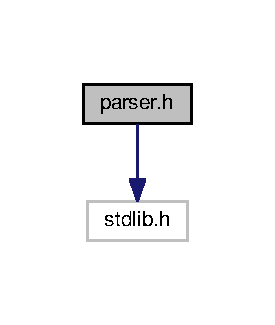
\includegraphics[width=132pt]{parser_8h__incl}
\end{center}
\end{figure}
This graph shows which files directly or indirectly include this file\+:
\nopagebreak
\begin{figure}[H]
\begin{center}
\leavevmode
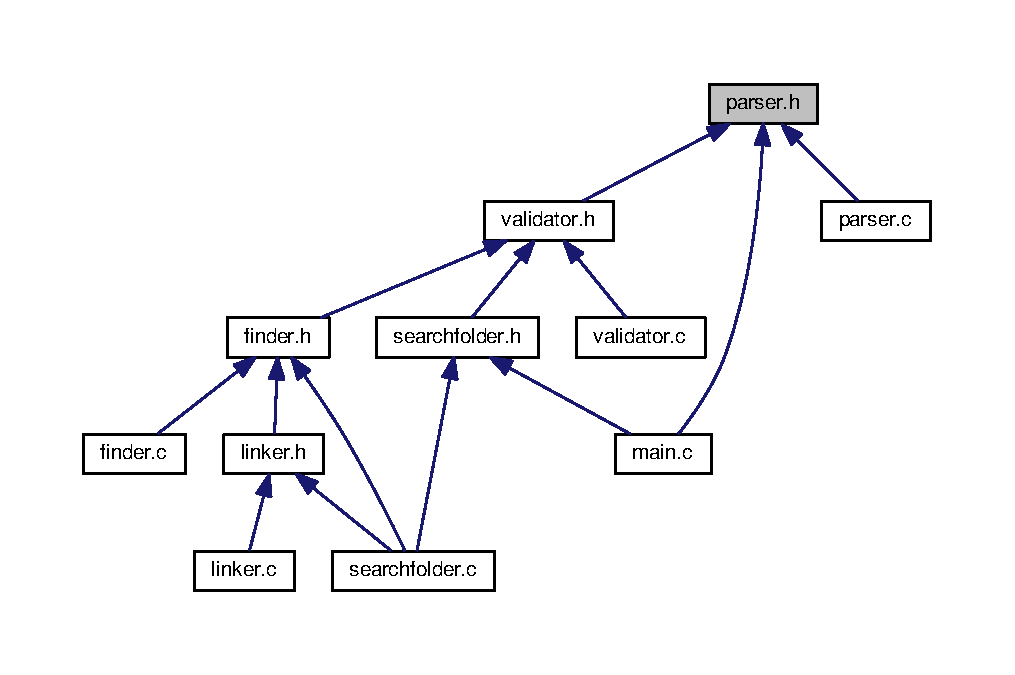
\includegraphics[width=350pt]{parser_8h__dep__incl}
\end{center}
\end{figure}
\subsection*{Data Structures}
\begin{DoxyCompactItemize}
\item 
struct \hyperlink{structparser__t}{parser\+\_\+t}
\begin{DoxyCompactList}\small\item\em Formal expression representation. \end{DoxyCompactList}\end{DoxyCompactItemize}
\subsection*{Typedefs}
\begin{DoxyCompactItemize}
\item 
typedef struct \hyperlink{structparser__t}{parser\+\_\+t} \hyperlink{parser_8h_a402117b92426b41469190a0d4d4397f0}{parser\+\_\+t}
\begin{DoxyCompactList}\small\item\em Formal expression representation. \end{DoxyCompactList}\end{DoxyCompactItemize}
\subsection*{Enumerations}
\begin{DoxyCompactItemize}
\item 
enum \hyperlink{parser_8h_a32088e9f194a33e050822b8c536e03cb}{parser\+\_\+crit\+\_\+type\+\_\+t} \{ {\bfseries O\+P\+E\+R\+A\+T\+OR} = 1 $<$$<$ 7, 
{\bfseries P\+A\+R\+E\+N\+T\+H\+E\+S\+IS} = 1 $<$$<$ 6, 
{\bfseries C\+R\+I\+T\+E\+R\+IA} = 1 $<$$<$ 5
 \}\begin{DoxyCompactList}\small\item\em Type of expression token. \end{DoxyCompactList}
\item 
enum \hyperlink{parser_8h_a4dcbe7148b91f50b0e7f3e08e780861d}{parser\+\_\+crit\+\_\+t} \{ \\*
{\bfseries OR} = O\+P\+E\+R\+A\+T\+OR, 
{\bfseries A\+ND}, 
{\bfseries N\+OT}, 
{\bfseries N\+A\+ME} = C\+R\+I\+T\+E\+R\+IA $\vert$ 3, 
\\*
{\bfseries U\+S\+ER}, 
{\bfseries G\+R\+O\+UP}, 
{\bfseries P\+E\+RM}, 
{\bfseries S\+I\+ZE}, 
\\*
{\bfseries A\+T\+I\+ME}, 
{\bfseries M\+T\+I\+ME}, 
{\bfseries C\+T\+I\+ME}, 
{\bfseries L\+P\+A\+R\+E\+N\+T\+H\+E\+S\+IS} = P\+A\+R\+E\+N\+T\+H\+E\+S\+IS, 
\\*
{\bfseries R\+P\+A\+R\+E\+N\+T\+H\+E\+S\+IS}
 \}\begin{DoxyCompactList}\small\item\em List of possible expression tokens. \end{DoxyCompactList}
\item 
enum \hyperlink{parser_8h_ac721d0db2049edef01e62a2e63ff0472}{parser\+\_\+comp\+\_\+t} \{ {\bfseries M\+AX}, 
{\bfseries M\+IN}, 
{\bfseries E\+X\+A\+CT}
 \}\begin{DoxyCompactList}\small\item\em The comparator used to evaluate criteria values. \end{DoxyCompactList}
\end{DoxyCompactItemize}
\subsection*{Functions}
\begin{DoxyCompactItemize}
\item 
\hyperlink{structparser__t}{parser\+\_\+t} $\ast$ \hyperlink{parser_8h_a570f8d50af35e4863518a619ef74d501}{parser\+\_\+parse} (char $\ast$expression\mbox{[}$\,$\mbox{]}, size\+\_\+t size)
\begin{DoxyCompactList}\small\item\em Parses the string expression, converting it to a {\ttfamily \hyperlink{structparser__t}{parser\+\_\+t}} representation. \end{DoxyCompactList}\item 
void \hyperlink{parser_8h_a680ceeada57c4645e365ba1745d41181}{parser\+\_\+free} (\hyperlink{structparser__t}{parser\+\_\+t} $\ast$expression)
\begin{DoxyCompactList}\small\item\em Frees the memory allocated for a {\ttfamily \hyperlink{structparser__t}{parser\+\_\+t}} instance. \end{DoxyCompactList}\end{DoxyCompactItemize}


\subsection{Detailed Description}
Parses a string expression and return a formal representation. 

Full unit test coverage 

\subsection{Typedef Documentation}
\index{parser.\+h@{parser.\+h}!parser\+\_\+t@{parser\+\_\+t}}
\index{parser\+\_\+t@{parser\+\_\+t}!parser.\+h@{parser.\+h}}
\subsubsection[{\texorpdfstring{parser\+\_\+t}{parser_t}}]{\setlength{\rightskip}{0pt plus 5cm}typedef struct {\bf parser\+\_\+t}  {\bf parser\+\_\+t}}\hypertarget{parser_8h_a402117b92426b41469190a0d4d4397f0}{}\label{parser_8h_a402117b92426b41469190a0d4d4397f0}


Formal expression representation. 

Contains the formal representation of the parsed expression in a ordered chained list. Each instance contains the information about a parsed expression token and the pointer to the {\ttfamily next} parsed expression token.

The order of the tokens in the chained list is not the same as the in the original string representation. Is has been reordered to encoded the priority of the operators and parenthesis in a infix notation 

\subsection{Enumeration Type Documentation}
\index{parser.\+h@{parser.\+h}!parser\+\_\+comp\+\_\+t@{parser\+\_\+comp\+\_\+t}}
\index{parser\+\_\+comp\+\_\+t@{parser\+\_\+comp\+\_\+t}!parser.\+h@{parser.\+h}}
\subsubsection[{\texorpdfstring{parser\+\_\+comp\+\_\+t}{parser_comp_t}}]{\setlength{\rightskip}{0pt plus 5cm}enum {\bf parser\+\_\+comp\+\_\+t}}\hypertarget{parser_8h_ac721d0db2049edef01e62a2e63ff0472}{}\label{parser_8h_ac721d0db2049edef01e62a2e63ff0472}


The comparator used to evaluate criteria values. 

Calculated for criteria that accepts the  in the values.
\begin{DoxyItemize}
\item Example\+: {\ttfamily -\/\+S\+I\+ZE +20k} or {\ttfamily -\/\+N\+A\+ME -\/.\+txt}
\end{DoxyItemize}

\begin{DoxySeeAlso}{See also}
\hyperlink{structparser__t}{parser\+\_\+t} 
\end{DoxySeeAlso}


Definition at line 60 of file parser.\+h.

\index{parser.\+h@{parser.\+h}!parser\+\_\+crit\+\_\+t@{parser\+\_\+crit\+\_\+t}}
\index{parser\+\_\+crit\+\_\+t@{parser\+\_\+crit\+\_\+t}!parser.\+h@{parser.\+h}}
\subsubsection[{\texorpdfstring{parser\+\_\+crit\+\_\+t}{parser_crit_t}}]{\setlength{\rightskip}{0pt plus 5cm}enum {\bf parser\+\_\+crit\+\_\+t}}\hypertarget{parser_8h_a4dcbe7148b91f50b0e7f3e08e780861d}{}\label{parser_8h_a4dcbe7148b91f50b0e7f3e08e780861d}


List of possible expression tokens. 

The enum values encode information\+:
\begin{DoxyItemize}
\item the 3 most significant bits hold the category (operator, criteria or parenthesis)
\item the 4 least significant bits hold the token order
\begin{DoxyItemize}
\item must start at 0 and be consecutive
\end{DoxyItemize}
\item operators are listed by priority A\+SC
\begin{DoxyItemize}
\item the encoded priority information is used in the parsing algorithm
\end{DoxyItemize}
\end{DoxyItemize}

\begin{DoxySeeAlso}{See also}
\hyperlink{parser_8h_a32088e9f194a33e050822b8c536e03cb}{parser\+\_\+crit\+\_\+type\+\_\+t} 

\hyperlink{structparser__t}{parser\+\_\+t} 
\end{DoxySeeAlso}


Definition at line 37 of file parser.\+h.

\index{parser.\+h@{parser.\+h}!parser\+\_\+crit\+\_\+type\+\_\+t@{parser\+\_\+crit\+\_\+type\+\_\+t}}
\index{parser\+\_\+crit\+\_\+type\+\_\+t@{parser\+\_\+crit\+\_\+type\+\_\+t}!parser.\+h@{parser.\+h}}
\subsubsection[{\texorpdfstring{parser\+\_\+crit\+\_\+type\+\_\+t}{parser_crit_type_t}}]{\setlength{\rightskip}{0pt plus 5cm}enum {\bf parser\+\_\+crit\+\_\+type\+\_\+t}}\hypertarget{parser_8h_a32088e9f194a33e050822b8c536e03cb}{}\label{parser_8h_a32088e9f194a33e050822b8c536e03cb}


Type of expression token. 

Used to flag bitwise the {\ttfamily parser\+\_\+crit\+\_\+t} enum values, and later to obtain the category of a given {\ttfamily parser\+\_\+crit\+\_\+t} enum value

\begin{DoxySeeAlso}{See also}
\hyperlink{parser_8h_a4dcbe7148b91f50b0e7f3e08e780861d}{parser\+\_\+crit\+\_\+t} 
\end{DoxySeeAlso}


Definition at line 19 of file parser.\+h.



\subsection{Function Documentation}
\index{parser.\+h@{parser.\+h}!parser\+\_\+free@{parser\+\_\+free}}
\index{parser\+\_\+free@{parser\+\_\+free}!parser.\+h@{parser.\+h}}
\subsubsection[{\texorpdfstring{parser\+\_\+free(parser\+\_\+t $\ast$expression)}{parser_free(parser_t *expression)}}]{\setlength{\rightskip}{0pt plus 5cm}void parser\+\_\+free (
\begin{DoxyParamCaption}
\item[{{\bf parser\+\_\+t} $\ast$}]{expression}
\end{DoxyParamCaption}
)}\hypertarget{parser_8h_a680ceeada57c4645e365ba1745d41181}{}\label{parser_8h_a680ceeada57c4645e365ba1745d41181}


Frees the memory allocated for a {\ttfamily \hyperlink{structparser__t}{parser\+\_\+t}} instance. 

\begin{DoxySeeAlso}{See also}
\hyperlink{structparser__t}{parser\+\_\+t} 
\end{DoxySeeAlso}

\begin{DoxyParams}{Parameters}
{\em expression} & The `parser\+\_\+t instance to free \\
\hline
\end{DoxyParams}


Definition at line 366 of file parser.\+c.

\index{parser.\+h@{parser.\+h}!parser\+\_\+parse@{parser\+\_\+parse}}
\index{parser\+\_\+parse@{parser\+\_\+parse}!parser.\+h@{parser.\+h}}
\subsubsection[{\texorpdfstring{parser\+\_\+parse(char $\ast$expression[], size\+\_\+t size)}{parser_parse(char *expression[], size_t size)}}]{\setlength{\rightskip}{0pt plus 5cm}{\bf parser\+\_\+t}$\ast$ parser\+\_\+parse (
\begin{DoxyParamCaption}
\item[{char $\ast$}]{expression\mbox{[}$\,$\mbox{]}, }
\item[{size\+\_\+t}]{size}
\end{DoxyParamCaption}
)}\hypertarget{parser_8h_a570f8d50af35e4863518a619ef74d501}{}\label{parser_8h_a570f8d50af35e4863518a619ef74d501}


Parses the string expression, converting it to a {\ttfamily \hyperlink{structparser__t}{parser\+\_\+t}} representation. 

This is done in multiple steps\+:
\begin{DoxyEnumerate}
\item tokens syntax is verified
\item criteria values units and comparison characters are verified
\item a object representation is created for each token
\item tokens are reordered to an infix notation encoding the operators priority and parenthesis
\end{DoxyEnumerate}

The algorithm used in step {\itshape 4} is based on the \href{https://en.wikipedia.org/wiki/Shunting-yard_algorithm}{\tt Shunting yard algorithm} (by Edsger Dijkstra). The original algorithm is intended to parse mathematical expressions and was adapt to parse our boolean expressions. \begin{DoxySeeAlso}{See also}
\hyperlink{structparser__t}{parser\+\_\+t}
\end{DoxySeeAlso}

\begin{DoxyParams}{Parameters}
{\em expression} & The list of tokens forming the expression (space splitted) \\
\hline
{\em size} & The number of elements in {\ttfamily expression} \\
\hline
\end{DoxyParams}
\begin{DoxyReturn}{Returns}
A {\ttfamily \hyperlink{structparser__t}{parser\+\_\+t}} representation of the expression, or {\itshape N\+U\+LL} is the expression is invalid 
\end{DoxyReturn}


Definition at line 339 of file parser.\+c.


\hypertarget{validator_8c}{}\section{/home/claudio/git/smart-\/folder/src/validator.c File Reference}
\label{validator_8c}\index{/home/claudio/git/smart-\/folder/src/validator.\+c@{/home/claudio/git/smart-\/folder/src/validator.\+c}}


Critera and operator evaludation functions.  


{\ttfamily \#include $<$string.\+h$>$}\\*
{\ttfamily \#include $<$time.\+h$>$}\\*
{\ttfamily \#include $<$sys/types.\+h$>$}\\*
{\ttfamily \#include \char`\"{}validator.\+h\char`\"{}}\\*
{\ttfamily \#include \char`\"{}logger.\+h\char`\"{}}\\*
Include dependency graph for validator.\+c\+:\nopagebreak
\begin{figure}[H]
\begin{center}
\leavevmode
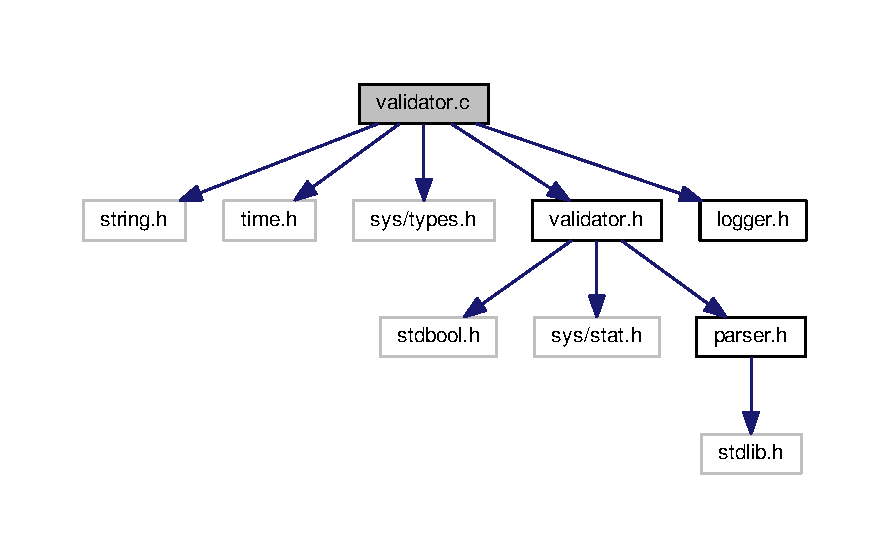
\includegraphics[width=350pt]{validator_8c__incl}
\end{center}
\end{figure}
\subsection*{Macros}
\begin{DoxyCompactItemize}
\item 
\#define \hyperlink{validator_8c_a20f8a4e237e6918372da5e1aec3426c8}{C\+R\+I\+T\+E\+R\+I\+A\+\_\+\+C\+O\+U\+NT}~11\hypertarget{validator_8c_a20f8a4e237e6918372da5e1aec3426c8}{}\label{validator_8c_a20f8a4e237e6918372da5e1aec3426c8}

\begin{DoxyCompactList}\small\item\em Number of criteria/operators. \end{DoxyCompactList}\item 
\#define \hyperlink{validator_8c_abe2627a9935b96daef8d9a2478934647}{P\+E\+R\+M\+\_\+\+O\+P\+T\+I\+O\+N\+S\+\_\+\+C\+O\+U\+NT}~9\hypertarget{validator_8c_abe2627a9935b96daef8d9a2478934647}{}\label{validator_8c_abe2627a9935b96daef8d9a2478934647}

\begin{DoxyCompactList}\small\item\em Number of permission options. \end{DoxyCompactList}\item 
\#define \hyperlink{validator_8c_a77d91bcc6068803c9eff253b1028073e}{C\+R\+I\+T\+E\+R\+I\+A\+\_\+\+O\+R\+D\+E\+R\+\_\+\+M\+A\+SK}~0b1111
\begin{DoxyCompactList}\small\item\em Mask that to apply to {\ttfamily parser\+\_\+crit\+\_\+t} to get criteria index in the enum. \end{DoxyCompactList}\end{DoxyCompactItemize}
\subsection*{Typedefs}
\begin{DoxyCompactItemize}
\item 
typedef bool($\ast$ \hyperlink{validator_8c_ad99afbcae8ae7f7cfee6a97184d5861b}{validate\+\_\+fn\+\_\+t}) (char $\ast$, struct stat $\ast$, \hyperlink{structparser__t}{parser\+\_\+t} $\ast$)\hypertarget{validator_8c_ad99afbcae8ae7f7cfee6a97184d5861b}{}\label{validator_8c_ad99afbcae8ae7f7cfee6a97184d5861b}

\begin{DoxyCompactList}\small\item\em Function pointer for criteria validate functions. \end{DoxyCompactList}\end{DoxyCompactItemize}
\subsection*{Enumerations}
\begin{DoxyCompactItemize}
\item 
enum \hyperlink{validator_8c_a156f9580ff03fe2c43a04418b103e97c}{validate\+\_\+perm\+\_\+type\+\_\+t} \{ {\bfseries R} = 4, 
{\bfseries W} = 2, 
{\bfseries X} = 1
 \}\begin{DoxyCompactList}\small\item\em List of permission types. \end{DoxyCompactList}
\item 
enum \hyperlink{validator_8c_a5de95e832572a2d519fc383840461239}{validate\+\_\+perm\+\_\+owner\+\_\+t} \{ {\bfseries U} = 6, 
{\bfseries G} = 3, 
{\bfseries O} = 0
 \}\begin{DoxyCompactList}\small\item\em List of permission targets. \end{DoxyCompactList}
\end{DoxyCompactItemize}
\subsection*{Functions}
\begin{DoxyCompactItemize}
\item 
static bool \hyperlink{validator_8c_a862284e5fc7d85e05483740c503ef148}{validate\+\_\+exp\+\_\+token} (char $\ast$filename, struct stat $\ast$filestat, \hyperlink{structparser__t}{parser\+\_\+t} $\ast$exp)
\begin{DoxyCompactList}\small\item\em Validates an expression token. \end{DoxyCompactList}\item 
static bool \hyperlink{validator_8c_adaa4bce57cef9baefdf7746d43e0c213}{validate\+\_\+or} (char $\ast$filename, struct stat $\ast$filestat, \hyperlink{structparser__t}{parser\+\_\+t} $\ast$exp)
\begin{DoxyCompactList}\small\item\em Validates OR operators. \end{DoxyCompactList}\item 
static bool \hyperlink{validator_8c_a95a034664a3f37186e065b898fc3d041}{validate\+\_\+and} (char $\ast$filename, struct stat $\ast$filestat, \hyperlink{structparser__t}{parser\+\_\+t} $\ast$exp)
\begin{DoxyCompactList}\small\item\em Validates A\+ND operators. \end{DoxyCompactList}\item 
static bool \hyperlink{validator_8c_a8341e1b958e2ec8cd5d5167212473731}{validate\+\_\+not} (char $\ast$filename, struct stat $\ast$filestat, \hyperlink{structparser__t}{parser\+\_\+t} $\ast$exp)
\begin{DoxyCompactList}\small\item\em Validates N\+OT operators. \end{DoxyCompactList}\item 
static bool \hyperlink{validator_8c_abd410628fdfe4e5df774cc57c13fa88e}{validate\+\_\+name} (char $\ast$filename, struct stat $\ast$filestat, \hyperlink{structparser__t}{parser\+\_\+t} $\ast$exp)
\begin{DoxyCompactList}\small\item\em Validates N\+A\+ME criteria. \end{DoxyCompactList}\item 
static bool \hyperlink{validator_8c_adca99e4146bc36bfb1ea9cd6a1335801}{validate\+\_\+user} (char $\ast$filename, struct stat $\ast$filestat, \hyperlink{structparser__t}{parser\+\_\+t} $\ast$exp)
\begin{DoxyCompactList}\small\item\em Validates U\+S\+ER criteria. \end{DoxyCompactList}\item 
static bool \hyperlink{validator_8c_a372b7bb2456d5211c7dac83eaaa4aec1}{validate\+\_\+group} (char $\ast$filename, struct stat $\ast$filestat, \hyperlink{structparser__t}{parser\+\_\+t} $\ast$exp)
\begin{DoxyCompactList}\small\item\em Validates G\+R\+O\+UP criteria. \end{DoxyCompactList}\item 
static bool \hyperlink{validator_8c_ab8e50ae831fd783fc9d455494d26b905}{validate\+\_\+perm} (char $\ast$filename, struct stat $\ast$filestat, \hyperlink{structparser__t}{parser\+\_\+t} $\ast$exp)
\begin{DoxyCompactList}\small\item\em Validates P\+E\+RM criteria. \end{DoxyCompactList}\item 
static bool \hyperlink{validator_8c_aa410d57420af99c3bdf2e174f3ab3321}{validate\+\_\+size} (char $\ast$filename, struct stat $\ast$filestat, \hyperlink{structparser__t}{parser\+\_\+t} $\ast$exp)
\begin{DoxyCompactList}\small\item\em Validates S\+I\+ZE criteria. \end{DoxyCompactList}\item 
static bool \hyperlink{validator_8c_a09e5b757b61865f2fe4f913e476db459}{validate\+\_\+time} (time\+\_\+t comp\+\_\+time, parser\+\_\+comp\+\_\+t comp, long refseconds)
\begin{DoxyCompactList}\small\item\em Factorizes time related validation. \end{DoxyCompactList}\item 
static bool \hyperlink{validator_8c_a8ca6f2c0ab321df18548c3e12c87b703}{validate\+\_\+atime} (char $\ast$filename, struct stat $\ast$filestat, \hyperlink{structparser__t}{parser\+\_\+t} $\ast$exp)
\begin{DoxyCompactList}\small\item\em Validates A\+T\+I\+ME criteria. \end{DoxyCompactList}\item 
static bool \hyperlink{validator_8c_aee84fd5cf26129acf79e7dfd2a5185c1}{validate\+\_\+mtime} (char $\ast$filename, struct stat $\ast$filestat, \hyperlink{structparser__t}{parser\+\_\+t} $\ast$exp)
\begin{DoxyCompactList}\small\item\em Validates M\+T\+I\+ME criteria. \end{DoxyCompactList}\item 
static bool \hyperlink{validator_8c_aa717edec98675daa659c16a1e51d2fc0}{validate\+\_\+ctime} (char $\ast$filename, struct stat $\ast$filestat, \hyperlink{structparser__t}{parser\+\_\+t} $\ast$exp)
\begin{DoxyCompactList}\small\item\em Validates C\+T\+I\+ME criteria. \end{DoxyCompactList}\item 
bool \hyperlink{validator_8c_aa0281da3748596d0f34db26d16661771}{validator\+\_\+validate} (char $\ast$filename, struct stat $\ast$filestat, \hyperlink{structparser__t}{parser\+\_\+t} $\ast$exp)
\begin{DoxyCompactList}\small\item\em Validates a file against an expression. \end{DoxyCompactList}\end{DoxyCompactItemize}
\subsection*{Variables}
\begin{DoxyCompactItemize}
\item 
static int \hyperlink{validator_8c_a59a13bfa9a783bc3c4d64cc8671db7ba}{P\+E\+R\+M\+\_\+\+O\+P\+T\+I\+O\+NS} \mbox{[}\hyperlink{validator_8c_abe2627a9935b96daef8d9a2478934647}{P\+E\+R\+M\+\_\+\+O\+P\+T\+I\+O\+N\+S\+\_\+\+C\+O\+U\+NT}\mbox{]} = \{R $<$$<$ U, W $<$$<$ U, X $<$$<$ U, R $<$$<$ G, W $<$$<$ G, X $<$$<$ G, R $<$$<$ O, W $<$$<$ O, X $<$$<$ O\}
\begin{DoxyCompactList}\small\item\em List of all permission options. \end{DoxyCompactList}\item 
static int \hyperlink{validator_8c_a119982f507a1f4dbe52025a97a127f9f}{P\+E\+R\+M\+\_\+\+F\+L\+A\+GS} \mbox{[}\hyperlink{validator_8c_abe2627a9935b96daef8d9a2478934647}{P\+E\+R\+M\+\_\+\+O\+P\+T\+I\+O\+N\+S\+\_\+\+C\+O\+U\+NT}\mbox{]}
\begin{DoxyCompactList}\small\item\em List of all \href{http://pubs.opengroup.org/onlinepubs/7908799/xsh/sysstat.h.html}{\tt OS permission flags} matching the permission options. \end{DoxyCompactList}\item 
static \hyperlink{validator_8c_ad99afbcae8ae7f7cfee6a97184d5861b}{validate\+\_\+fn\+\_\+t} \hyperlink{validator_8c_a9839e177025c582f4ad9d7c007141636}{validators} \mbox{[}\hyperlink{validator_8c_a20f8a4e237e6918372da5e1aec3426c8}{C\+R\+I\+T\+E\+R\+I\+A\+\_\+\+C\+O\+U\+NT}\mbox{]}
\begin{DoxyCompactList}\small\item\em List of of criteria validate functions. \end{DoxyCompactList}\end{DoxyCompactItemize}


\subsection{Detailed Description}
Critera and operator evaludation functions. 

Contains the logic to evaluate each possible critera and operator. 

\subsection{Macro Definition Documentation}
\index{validator.\+c@{validator.\+c}!C\+R\+I\+T\+E\+R\+I\+A\+\_\+\+O\+R\+D\+E\+R\+\_\+\+M\+A\+SK@{C\+R\+I\+T\+E\+R\+I\+A\+\_\+\+O\+R\+D\+E\+R\+\_\+\+M\+A\+SK}}
\index{C\+R\+I\+T\+E\+R\+I\+A\+\_\+\+O\+R\+D\+E\+R\+\_\+\+M\+A\+SK@{C\+R\+I\+T\+E\+R\+I\+A\+\_\+\+O\+R\+D\+E\+R\+\_\+\+M\+A\+SK}!validator.\+c@{validator.\+c}}
\subsubsection[{\texorpdfstring{C\+R\+I\+T\+E\+R\+I\+A\+\_\+\+O\+R\+D\+E\+R\+\_\+\+M\+A\+SK}{CRITERIA_ORDER_MASK}}]{\setlength{\rightskip}{0pt plus 5cm}\#define C\+R\+I\+T\+E\+R\+I\+A\+\_\+\+O\+R\+D\+E\+R\+\_\+\+M\+A\+SK~0b1111}\hypertarget{validator_8c_a77d91bcc6068803c9eff253b1028073e}{}\label{validator_8c_a77d91bcc6068803c9eff253b1028073e}


Mask that to apply to {\ttfamily parser\+\_\+crit\+\_\+t} to get criteria index in the enum. 

\begin{DoxySeeAlso}{See also}
parser\+\_\+crit\+\_\+t 
\end{DoxySeeAlso}


Definition at line 18 of file validator.\+c.



\subsection{Enumeration Type Documentation}
\index{validator.\+c@{validator.\+c}!validate\+\_\+perm\+\_\+owner\+\_\+t@{validate\+\_\+perm\+\_\+owner\+\_\+t}}
\index{validate\+\_\+perm\+\_\+owner\+\_\+t@{validate\+\_\+perm\+\_\+owner\+\_\+t}!validator.\+c@{validator.\+c}}
\subsubsection[{\texorpdfstring{validate\+\_\+perm\+\_\+owner\+\_\+t}{validate_perm_owner_t}}]{\setlength{\rightskip}{0pt plus 5cm}enum {\bf validate\+\_\+perm\+\_\+owner\+\_\+t}}\hypertarget{validator_8c_a5de95e832572a2d519fc383840461239}{}\label{validator_8c_a5de95e832572a2d519fc383840461239}


List of permission targets. 


\begin{DoxyItemize}
\item user
\item group
\item owner
\end{DoxyItemize}

Used to shift {\ttfamily validate\+\_\+perm\+\_\+type\+\_\+t} bitwise \begin{DoxySeeAlso}{See also}
\hyperlink{validator_8c_a156f9580ff03fe2c43a04418b103e97c}{validate\+\_\+perm\+\_\+type\+\_\+t} 
\end{DoxySeeAlso}


Definition at line 41 of file validator.\+c.

\index{validator.\+c@{validator.\+c}!validate\+\_\+perm\+\_\+type\+\_\+t@{validate\+\_\+perm\+\_\+type\+\_\+t}}
\index{validate\+\_\+perm\+\_\+type\+\_\+t@{validate\+\_\+perm\+\_\+type\+\_\+t}!validator.\+c@{validator.\+c}}
\subsubsection[{\texorpdfstring{validate\+\_\+perm\+\_\+type\+\_\+t}{validate_perm_type_t}}]{\setlength{\rightskip}{0pt plus 5cm}enum {\bf validate\+\_\+perm\+\_\+type\+\_\+t}}\hypertarget{validator_8c_a156f9580ff03fe2c43a04418b103e97c}{}\label{validator_8c_a156f9580ff03fe2c43a04418b103e97c}


List of permission types. 


\begin{DoxyItemize}
\item read
\item write
\item execute
\end{DoxyItemize}

\begin{DoxySeeAlso}{See also}
\hyperlink{validator_8c_a5de95e832572a2d519fc383840461239}{validate\+\_\+perm\+\_\+owner\+\_\+t} 
\end{DoxySeeAlso}


Definition at line 27 of file validator.\+c.



\subsection{Function Documentation}
\index{validator.\+c@{validator.\+c}!validate\+\_\+and@{validate\+\_\+and}}
\index{validate\+\_\+and@{validate\+\_\+and}!validator.\+c@{validator.\+c}}
\subsubsection[{\texorpdfstring{validate\+\_\+and(char $\ast$filename, struct stat $\ast$filestat, parser\+\_\+t $\ast$exp)}{validate_and(char *filename, struct stat *filestat, parser_t *exp)}}]{\setlength{\rightskip}{0pt plus 5cm}static bool validate\+\_\+and (
\begin{DoxyParamCaption}
\item[{char $\ast$}]{filename, }
\item[{struct stat $\ast$}]{filestat, }
\item[{{\bf parser\+\_\+t} $\ast$}]{exp}
\end{DoxyParamCaption}
)\hspace{0.3cm}{\ttfamily [static]}}\hypertarget{validator_8c_a95a034664a3f37186e065b898fc3d041}{}\label{validator_8c_a95a034664a3f37186e065b898fc3d041}


Validates A\+ND operators. 



Definition at line 72 of file validator.\+c.

\index{validator.\+c@{validator.\+c}!validate\+\_\+atime@{validate\+\_\+atime}}
\index{validate\+\_\+atime@{validate\+\_\+atime}!validator.\+c@{validator.\+c}}
\subsubsection[{\texorpdfstring{validate\+\_\+atime(char $\ast$filename, struct stat $\ast$filestat, parser\+\_\+t $\ast$exp)}{validate_atime(char *filename, struct stat *filestat, parser_t *exp)}}]{\setlength{\rightskip}{0pt plus 5cm}static bool validate\+\_\+atime (
\begin{DoxyParamCaption}
\item[{char $\ast$}]{filename, }
\item[{struct stat $\ast$}]{filestat, }
\item[{{\bf parser\+\_\+t} $\ast$}]{exp}
\end{DoxyParamCaption}
)\hspace{0.3cm}{\ttfamily [static]}}\hypertarget{validator_8c_a8ca6f2c0ab321df18548c3e12c87b703}{}\label{validator_8c_a8ca6f2c0ab321df18548c3e12c87b703}


Validates A\+T\+I\+ME criteria. 



Definition at line 131 of file validator.\+c.

\index{validator.\+c@{validator.\+c}!validate\+\_\+ctime@{validate\+\_\+ctime}}
\index{validate\+\_\+ctime@{validate\+\_\+ctime}!validator.\+c@{validator.\+c}}
\subsubsection[{\texorpdfstring{validate\+\_\+ctime(char $\ast$filename, struct stat $\ast$filestat, parser\+\_\+t $\ast$exp)}{validate_ctime(char *filename, struct stat *filestat, parser_t *exp)}}]{\setlength{\rightskip}{0pt plus 5cm}static bool validate\+\_\+ctime (
\begin{DoxyParamCaption}
\item[{char $\ast$}]{filename, }
\item[{struct stat $\ast$}]{filestat, }
\item[{{\bf parser\+\_\+t} $\ast$}]{exp}
\end{DoxyParamCaption}
)\hspace{0.3cm}{\ttfamily [static]}}\hypertarget{validator_8c_aa717edec98675daa659c16a1e51d2fc0}{}\label{validator_8c_aa717edec98675daa659c16a1e51d2fc0}


Validates C\+T\+I\+ME criteria. 



Definition at line 143 of file validator.\+c.

\index{validator.\+c@{validator.\+c}!validate\+\_\+exp\+\_\+token@{validate\+\_\+exp\+\_\+token}}
\index{validate\+\_\+exp\+\_\+token@{validate\+\_\+exp\+\_\+token}!validator.\+c@{validator.\+c}}
\subsubsection[{\texorpdfstring{validate\+\_\+exp\+\_\+token(char $\ast$filename, struct stat $\ast$filestat, parser\+\_\+t $\ast$exp)}{validate_exp_token(char *filename, struct stat *filestat, parser_t *exp)}}]{\setlength{\rightskip}{0pt plus 5cm}static bool validate\+\_\+exp\+\_\+token (
\begin{DoxyParamCaption}
\item[{char $\ast$}]{filename, }
\item[{struct stat $\ast$}]{filestat, }
\item[{{\bf parser\+\_\+t} $\ast$}]{exp}
\end{DoxyParamCaption}
)\hspace{0.3cm}{\ttfamily [static]}}\hypertarget{validator_8c_a862284e5fc7d85e05483740c503ef148}{}\label{validator_8c_a862284e5fc7d85e05483740c503ef148}


Validates an expression token. 

Retrieves the validate function corrsponding to the expression token, which can be a criteria or an operator 

Definition at line 169 of file validator.\+c.

\index{validator.\+c@{validator.\+c}!validate\+\_\+group@{validate\+\_\+group}}
\index{validate\+\_\+group@{validate\+\_\+group}!validator.\+c@{validator.\+c}}
\subsubsection[{\texorpdfstring{validate\+\_\+group(char $\ast$filename, struct stat $\ast$filestat, parser\+\_\+t $\ast$exp)}{validate_group(char *filename, struct stat *filestat, parser_t *exp)}}]{\setlength{\rightskip}{0pt plus 5cm}static bool validate\+\_\+group (
\begin{DoxyParamCaption}
\item[{char $\ast$}]{filename, }
\item[{struct stat $\ast$}]{filestat, }
\item[{{\bf parser\+\_\+t} $\ast$}]{exp}
\end{DoxyParamCaption}
)\hspace{0.3cm}{\ttfamily [static]}}\hypertarget{validator_8c_a372b7bb2456d5211c7dac83eaaa4aec1}{}\label{validator_8c_a372b7bb2456d5211c7dac83eaaa4aec1}


Validates G\+R\+O\+UP criteria. 



Definition at line 96 of file validator.\+c.

\index{validator.\+c@{validator.\+c}!validate\+\_\+mtime@{validate\+\_\+mtime}}
\index{validate\+\_\+mtime@{validate\+\_\+mtime}!validator.\+c@{validator.\+c}}
\subsubsection[{\texorpdfstring{validate\+\_\+mtime(char $\ast$filename, struct stat $\ast$filestat, parser\+\_\+t $\ast$exp)}{validate_mtime(char *filename, struct stat *filestat, parser_t *exp)}}]{\setlength{\rightskip}{0pt plus 5cm}static bool validate\+\_\+mtime (
\begin{DoxyParamCaption}
\item[{char $\ast$}]{filename, }
\item[{struct stat $\ast$}]{filestat, }
\item[{{\bf parser\+\_\+t} $\ast$}]{exp}
\end{DoxyParamCaption}
)\hspace{0.3cm}{\ttfamily [static]}}\hypertarget{validator_8c_aee84fd5cf26129acf79e7dfd2a5185c1}{}\label{validator_8c_aee84fd5cf26129acf79e7dfd2a5185c1}


Validates M\+T\+I\+ME criteria. 



Definition at line 137 of file validator.\+c.

\index{validator.\+c@{validator.\+c}!validate\+\_\+name@{validate\+\_\+name}}
\index{validate\+\_\+name@{validate\+\_\+name}!validator.\+c@{validator.\+c}}
\subsubsection[{\texorpdfstring{validate\+\_\+name(char $\ast$filename, struct stat $\ast$filestat, parser\+\_\+t $\ast$exp)}{validate_name(char *filename, struct stat *filestat, parser_t *exp)}}]{\setlength{\rightskip}{0pt plus 5cm}static bool validate\+\_\+name (
\begin{DoxyParamCaption}
\item[{char $\ast$}]{filename, }
\item[{struct stat $\ast$}]{filestat, }
\item[{{\bf parser\+\_\+t} $\ast$}]{exp}
\end{DoxyParamCaption}
)\hspace{0.3cm}{\ttfamily [static]}}\hypertarget{validator_8c_abd410628fdfe4e5df774cc57c13fa88e}{}\label{validator_8c_abd410628fdfe4e5df774cc57c13fa88e}


Validates N\+A\+ME criteria. 



Definition at line 83 of file validator.\+c.

\index{validator.\+c@{validator.\+c}!validate\+\_\+not@{validate\+\_\+not}}
\index{validate\+\_\+not@{validate\+\_\+not}!validator.\+c@{validator.\+c}}
\subsubsection[{\texorpdfstring{validate\+\_\+not(char $\ast$filename, struct stat $\ast$filestat, parser\+\_\+t $\ast$exp)}{validate_not(char *filename, struct stat *filestat, parser_t *exp)}}]{\setlength{\rightskip}{0pt plus 5cm}static bool validate\+\_\+not (
\begin{DoxyParamCaption}
\item[{char $\ast$}]{filename, }
\item[{struct stat $\ast$}]{filestat, }
\item[{{\bf parser\+\_\+t} $\ast$}]{exp}
\end{DoxyParamCaption}
)\hspace{0.3cm}{\ttfamily [static]}}\hypertarget{validator_8c_a8341e1b958e2ec8cd5d5167212473731}{}\label{validator_8c_a8341e1b958e2ec8cd5d5167212473731}


Validates N\+OT operators. 



Definition at line 78 of file validator.\+c.

\index{validator.\+c@{validator.\+c}!validate\+\_\+or@{validate\+\_\+or}}
\index{validate\+\_\+or@{validate\+\_\+or}!validator.\+c@{validator.\+c}}
\subsubsection[{\texorpdfstring{validate\+\_\+or(char $\ast$filename, struct stat $\ast$filestat, parser\+\_\+t $\ast$exp)}{validate_or(char *filename, struct stat *filestat, parser_t *exp)}}]{\setlength{\rightskip}{0pt plus 5cm}static bool validate\+\_\+or (
\begin{DoxyParamCaption}
\item[{char $\ast$}]{filename, }
\item[{struct stat $\ast$}]{filestat, }
\item[{{\bf parser\+\_\+t} $\ast$}]{exp}
\end{DoxyParamCaption}
)\hspace{0.3cm}{\ttfamily [static]}}\hypertarget{validator_8c_adaa4bce57cef9baefdf7746d43e0c213}{}\label{validator_8c_adaa4bce57cef9baefdf7746d43e0c213}


Validates OR operators. 



Definition at line 66 of file validator.\+c.

\index{validator.\+c@{validator.\+c}!validate\+\_\+perm@{validate\+\_\+perm}}
\index{validate\+\_\+perm@{validate\+\_\+perm}!validator.\+c@{validator.\+c}}
\subsubsection[{\texorpdfstring{validate\+\_\+perm(char $\ast$filename, struct stat $\ast$filestat, parser\+\_\+t $\ast$exp)}{validate_perm(char *filename, struct stat *filestat, parser_t *exp)}}]{\setlength{\rightskip}{0pt plus 5cm}static bool validate\+\_\+perm (
\begin{DoxyParamCaption}
\item[{char $\ast$}]{filename, }
\item[{struct stat $\ast$}]{filestat, }
\item[{{\bf parser\+\_\+t} $\ast$}]{exp}
\end{DoxyParamCaption}
)\hspace{0.3cm}{\ttfamily [static]}}\hypertarget{validator_8c_ab8e50ae831fd783fc9d455494d26b905}{}\label{validator_8c_ab8e50ae831fd783fc9d455494d26b905}


Validates P\+E\+RM criteria. 



Definition at line 102 of file validator.\+c.

\index{validator.\+c@{validator.\+c}!validate\+\_\+size@{validate\+\_\+size}}
\index{validate\+\_\+size@{validate\+\_\+size}!validator.\+c@{validator.\+c}}
\subsubsection[{\texorpdfstring{validate\+\_\+size(char $\ast$filename, struct stat $\ast$filestat, parser\+\_\+t $\ast$exp)}{validate_size(char *filename, struct stat *filestat, parser_t *exp)}}]{\setlength{\rightskip}{0pt plus 5cm}static bool validate\+\_\+size (
\begin{DoxyParamCaption}
\item[{char $\ast$}]{filename, }
\item[{struct stat $\ast$}]{filestat, }
\item[{{\bf parser\+\_\+t} $\ast$}]{exp}
\end{DoxyParamCaption}
)\hspace{0.3cm}{\ttfamily [static]}}\hypertarget{validator_8c_aa410d57420af99c3bdf2e174f3ab3321}{}\label{validator_8c_aa410d57420af99c3bdf2e174f3ab3321}


Validates S\+I\+ZE criteria. 



Definition at line 117 of file validator.\+c.

\index{validator.\+c@{validator.\+c}!validate\+\_\+time@{validate\+\_\+time}}
\index{validate\+\_\+time@{validate\+\_\+time}!validator.\+c@{validator.\+c}}
\subsubsection[{\texorpdfstring{validate\+\_\+time(time\+\_\+t comp\+\_\+time, parser\+\_\+comp\+\_\+t comp, long refseconds)}{validate_time(time_t comp_time, parser_comp_t comp, long refseconds)}}]{\setlength{\rightskip}{0pt plus 5cm}static bool validate\+\_\+time (
\begin{DoxyParamCaption}
\item[{time\+\_\+t}]{comp\+\_\+time, }
\item[{parser\+\_\+comp\+\_\+t}]{comp, }
\item[{long}]{refseconds}
\end{DoxyParamCaption}
)\hspace{0.3cm}{\ttfamily [static]}}\hypertarget{validator_8c_a09e5b757b61865f2fe4f913e476db459}{}\label{validator_8c_a09e5b757b61865f2fe4f913e476db459}


Factorizes time related validation. 



Definition at line 124 of file validator.\+c.

\index{validator.\+c@{validator.\+c}!validate\+\_\+user@{validate\+\_\+user}}
\index{validate\+\_\+user@{validate\+\_\+user}!validator.\+c@{validator.\+c}}
\subsubsection[{\texorpdfstring{validate\+\_\+user(char $\ast$filename, struct stat $\ast$filestat, parser\+\_\+t $\ast$exp)}{validate_user(char *filename, struct stat *filestat, parser_t *exp)}}]{\setlength{\rightskip}{0pt plus 5cm}static bool validate\+\_\+user (
\begin{DoxyParamCaption}
\item[{char $\ast$}]{filename, }
\item[{struct stat $\ast$}]{filestat, }
\item[{{\bf parser\+\_\+t} $\ast$}]{exp}
\end{DoxyParamCaption}
)\hspace{0.3cm}{\ttfamily [static]}}\hypertarget{validator_8c_adca99e4146bc36bfb1ea9cd6a1335801}{}\label{validator_8c_adca99e4146bc36bfb1ea9cd6a1335801}


Validates U\+S\+ER criteria. 



Definition at line 90 of file validator.\+c.

\index{validator.\+c@{validator.\+c}!validator\+\_\+validate@{validator\+\_\+validate}}
\index{validator\+\_\+validate@{validator\+\_\+validate}!validator.\+c@{validator.\+c}}
\subsubsection[{\texorpdfstring{validator\+\_\+validate(char $\ast$filename, struct stat $\ast$filestat, parser\+\_\+t $\ast$exp)}{validator_validate(char *filename, struct stat *filestat, parser_t *exp)}}]{\setlength{\rightskip}{0pt plus 5cm}bool validator\+\_\+validate (
\begin{DoxyParamCaption}
\item[{char $\ast$}]{filename, }
\item[{struct stat $\ast$}]{filestat, }
\item[{{\bf parser\+\_\+t} $\ast$}]{exp}
\end{DoxyParamCaption}
)}\hypertarget{validator_8c_aa0281da3748596d0f34db26d16661771}{}\label{validator_8c_aa0281da3748596d0f34db26d16661771}


Validates a file against an expression. 



Definition at line 179 of file validator.\+c.



\subsection{Variable Documentation}
\index{validator.\+c@{validator.\+c}!P\+E\+R\+M\+\_\+\+F\+L\+A\+GS@{P\+E\+R\+M\+\_\+\+F\+L\+A\+GS}}
\index{P\+E\+R\+M\+\_\+\+F\+L\+A\+GS@{P\+E\+R\+M\+\_\+\+F\+L\+A\+GS}!validator.\+c@{validator.\+c}}
\subsubsection[{\texorpdfstring{P\+E\+R\+M\+\_\+\+F\+L\+A\+GS}{PERM_FLAGS}}]{\setlength{\rightskip}{0pt plus 5cm}int P\+E\+R\+M\+\_\+\+F\+L\+A\+GS\mbox{[}{\bf P\+E\+R\+M\+\_\+\+O\+P\+T\+I\+O\+N\+S\+\_\+\+C\+O\+U\+NT}\mbox{]}\hspace{0.3cm}{\ttfamily [static]}}\hypertarget{validator_8c_a119982f507a1f4dbe52025a97a127f9f}{}\label{validator_8c_a119982f507a1f4dbe52025a97a127f9f}
{\bfseries Initial value\+:}
\begin{DoxyCode}
= \{S\_IRUSR, S\_IWUSR, S\_IXUSR, S\_IRGRP, S\_IWGRP,
                                             S\_IXGRP, S\_IROTH, S\_IWOTH, S\_IXOTH\}
\end{DoxyCode}


List of all \href{http://pubs.opengroup.org/onlinepubs/7908799/xsh/sysstat.h.html}{\tt OS permission flags} matching the permission options. 

\begin{DoxySeeAlso}{See also}
\hyperlink{validator_8c_a156f9580ff03fe2c43a04418b103e97c}{validate\+\_\+perm\+\_\+type\+\_\+t} 

\hyperlink{validator_8c_a59a13bfa9a783bc3c4d64cc8671db7ba}{P\+E\+R\+M\+\_\+\+O\+P\+T\+I\+O\+NS} 
\end{DoxySeeAlso}


Definition at line 60 of file validator.\+c.

\index{validator.\+c@{validator.\+c}!P\+E\+R\+M\+\_\+\+O\+P\+T\+I\+O\+NS@{P\+E\+R\+M\+\_\+\+O\+P\+T\+I\+O\+NS}}
\index{P\+E\+R\+M\+\_\+\+O\+P\+T\+I\+O\+NS@{P\+E\+R\+M\+\_\+\+O\+P\+T\+I\+O\+NS}!validator.\+c@{validator.\+c}}
\subsubsection[{\texorpdfstring{P\+E\+R\+M\+\_\+\+O\+P\+T\+I\+O\+NS}{PERM_OPTIONS}}]{\setlength{\rightskip}{0pt plus 5cm}int P\+E\+R\+M\+\_\+\+O\+P\+T\+I\+O\+NS\mbox{[}{\bf P\+E\+R\+M\+\_\+\+O\+P\+T\+I\+O\+N\+S\+\_\+\+C\+O\+U\+NT}\mbox{]} = \{R $<$$<$ U, W $<$$<$ U, X $<$$<$ U, R $<$$<$ G, W $<$$<$ G, X $<$$<$ G, R $<$$<$ O, W $<$$<$ O, X $<$$<$ O\}\hspace{0.3cm}{\ttfamily [static]}}\hypertarget{validator_8c_a59a13bfa9a783bc3c4d64cc8671db7ba}{}\label{validator_8c_a59a13bfa9a783bc3c4d64cc8671db7ba}


List of all permission options. 

Composed by combining {\ttfamily validate\+\_\+perm\+\_\+type\+\_\+t} and {\ttfamily validate\+\_\+perm\+\_\+owner\+\_\+t} \begin{DoxySeeAlso}{See also}
\hyperlink{validator_8c_a156f9580ff03fe2c43a04418b103e97c}{validate\+\_\+perm\+\_\+type\+\_\+t} 

\hyperlink{validator_8c_a5de95e832572a2d519fc383840461239}{validate\+\_\+perm\+\_\+owner\+\_\+t} 
\end{DoxySeeAlso}


Definition at line 53 of file validator.\+c.

\index{validator.\+c@{validator.\+c}!validators@{validators}}
\index{validators@{validators}!validator.\+c@{validator.\+c}}
\subsubsection[{\texorpdfstring{validators}{validators}}]{\setlength{\rightskip}{0pt plus 5cm}{\bf validate\+\_\+fn\+\_\+t} validators\mbox{[}{\bf C\+R\+I\+T\+E\+R\+I\+A\+\_\+\+C\+O\+U\+NT}\mbox{]}\hspace{0.3cm}{\ttfamily [static]}}\hypertarget{validator_8c_a9839e177025c582f4ad9d7c007141636}{}\label{validator_8c_a9839e177025c582f4ad9d7c007141636}
{\bfseries Initial value\+:}
\begin{DoxyCode}
= \{&\hyperlink{validator_8c_adaa4bce57cef9baefdf7746d43e0c213}{validate\_or},    &\hyperlink{validator_8c_a95a034664a3f37186e065b898fc3d041}{validate\_and},   &\hyperlink{validator_8c_a8341e1b958e2ec8cd5d5167212473731}{validate\_not},  &
      \hyperlink{validator_8c_abd410628fdfe4e5df774cc57c13fa88e}{validate\_name},
                                                   &\hyperlink{validator_8c_adca99e4146bc36bfb1ea9cd6a1335801}{validate\_user},  &
      \hyperlink{validator_8c_a372b7bb2456d5211c7dac83eaaa4aec1}{validate\_group}, &\hyperlink{validator_8c_ab8e50ae831fd783fc9d455494d26b905}{validate\_perm}, &\hyperlink{validator_8c_aa410d57420af99c3bdf2e174f3ab3321}{validate\_size},
                                                   &\hyperlink{validator_8c_a8ca6f2c0ab321df18548c3e12c87b703}{validate\_atime}, &
      \hyperlink{validator_8c_aee84fd5cf26129acf79e7dfd2a5185c1}{validate\_mtime}, &\hyperlink{validator_8c_aa717edec98675daa659c16a1e51d2fc0}{validate\_ctime}\}
\end{DoxyCode}


List of of criteria validate functions. 

Array contained the list of all the criteria specific validate functions The order is important as it must match the index of the criteria in {\ttfamily parser\+\_\+crit\+\_\+t}

\begin{DoxySeeAlso}{See also}
parser\+\_\+crit\+\_\+t 

\hyperlink{validator_8c_ad99afbcae8ae7f7cfee6a97184d5861b}{validate\+\_\+fn\+\_\+t} 

\hyperlink{validator_8c_a77d91bcc6068803c9eff253b1028073e}{C\+R\+I\+T\+E\+R\+I\+A\+\_\+\+O\+R\+D\+E\+R\+\_\+\+M\+A\+SK} 
\end{DoxySeeAlso}


Definition at line 160 of file validator.\+c.


\hypertarget{validator_8h}{}\section{validator.\+h File Reference}
\label{validator_8h}\index{validator.\+h@{validator.\+h}}


Validates files against a parsed criteria expression.  


{\ttfamily \#include $<$stdbool.\+h$>$}\\*
{\ttfamily \#include $<$sys/stat.\+h$>$}\\*
{\ttfamily \#include \char`\"{}parser.\+h\char`\"{}}\\*
Include dependency graph for validator.\+h\+:\nopagebreak
\begin{figure}[H]
\begin{center}
\leavevmode
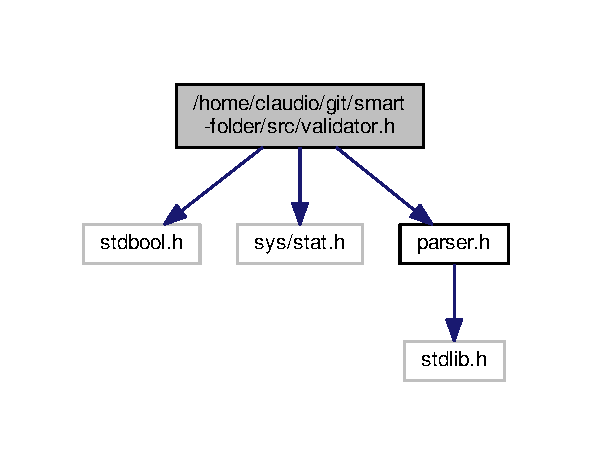
\includegraphics[width=284pt]{validator_8h__incl}
\end{center}
\end{figure}
This graph shows which files directly or indirectly include this file\+:
\nopagebreak
\begin{figure}[H]
\begin{center}
\leavevmode
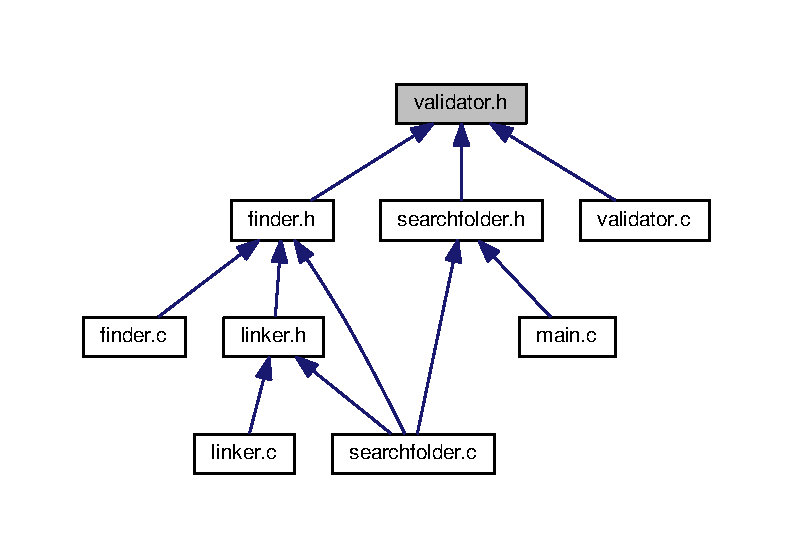
\includegraphics[width=350pt]{validator_8h__dep__incl}
\end{center}
\end{figure}
\subsection*{Functions}
\begin{DoxyCompactItemize}
\item 
bool \hyperlink{validator_8h_a0abc93342b9898145ea067c4a538022a}{validator\+\_\+validate} (char $\ast$filename, struct stat $\ast$filestat, \hyperlink{structparser__t}{parser\+\_\+t} $\ast$expression)
\begin{DoxyCompactList}\small\item\em Validates a file against an expression. \end{DoxyCompactList}\end{DoxyCompactItemize}


\subsection{Detailed Description}
Validates files against a parsed criteria expression. 



\subsection{Function Documentation}
\index{validator.\+h@{validator.\+h}!validator\+\_\+validate@{validator\+\_\+validate}}
\index{validator\+\_\+validate@{validator\+\_\+validate}!validator.\+h@{validator.\+h}}
\subsubsection[{\texorpdfstring{validator\+\_\+validate(char $\ast$filename, struct stat $\ast$filestat, parser\+\_\+t $\ast$expression)}{validator_validate(char *filename, struct stat *filestat, parser_t *expression)}}]{\setlength{\rightskip}{0pt plus 5cm}bool validator\+\_\+validate (
\begin{DoxyParamCaption}
\item[{char $\ast$}]{filename, }
\item[{struct stat $\ast$}]{filestat, }
\item[{{\bf parser\+\_\+t} $\ast$}]{exp}
\end{DoxyParamCaption}
)}\hypertarget{validator_8h_a0abc93342b9898145ea067c4a538022a}{}\label{validator_8h_a0abc93342b9898145ea067c4a538022a}


Validates a file against an expression. 


\begin{DoxyParams}{Parameters}
{\em filename} & The file\textquotesingle{}s name \\
\hline
{\em filestat} & The file\textquotesingle{}s attributes \\
\hline
{\em expression} & The expression used to validate the file \\
\hline
\end{DoxyParams}
\begin{DoxyReturn}{Returns}
If the file is valid
\end{DoxyReturn}


Definition at line 179 of file validator.\+c.


%--- End generated contents ---

% Index
\backmatter
\newpage
\phantomsection
\clearemptydoublepage
\addcontentsline{toc}{chapter}{Index}
\printindex

\end{document}
